% Options for packages loaded elsewhere
\PassOptionsToPackage{unicode}{hyperref}
\PassOptionsToPackage{hyphens}{url}
%
\documentclass[
  12pt,
  a4paper,
]{article}
\usepackage{amsmath,amssymb}
\usepackage{setspace}
\usepackage{iftex}
\ifPDFTeX
  \usepackage[T1]{fontenc}
  \usepackage[utf8]{inputenc}
  \usepackage{textcomp} % provide euro and other symbols
\else % if luatex or xetex
  \usepackage{unicode-math} % this also loads fontspec
  \defaultfontfeatures{Scale=MatchLowercase}
  \defaultfontfeatures[\rmfamily]{Ligatures=TeX,Scale=1}
\fi
\usepackage{lmodern}
\ifPDFTeX\else
  % xetex/luatex font selection
\fi
% Use upquote if available, for straight quotes in verbatim environments
\IfFileExists{upquote.sty}{\usepackage{upquote}}{}
\IfFileExists{microtype.sty}{% use microtype if available
  \usepackage[]{microtype}
  \UseMicrotypeSet[protrusion]{basicmath} % disable protrusion for tt fonts
}{}
\makeatletter
\@ifundefined{KOMAClassName}{% if non-KOMA class
  \IfFileExists{parskip.sty}{%
    \usepackage{parskip}
  }{% else
    \setlength{\parindent}{0pt}
    \setlength{\parskip}{6pt plus 2pt minus 1pt}}
}{% if KOMA class
  \KOMAoptions{parskip=half}}
\makeatother
\usepackage{xcolor}
\usepackage[top=2cm,bottom=2cm,left=3cm,right=1.5cm]{geometry}
\usepackage{graphicx}
\makeatletter
\def\maxwidth{\ifdim\Gin@nat@width>\linewidth\linewidth\else\Gin@nat@width\fi}
\def\maxheight{\ifdim\Gin@nat@height>\textheight\textheight\else\Gin@nat@height\fi}
\makeatother
% Scale images if necessary, so that they will not overflow the page
% margins by default, and it is still possible to overwrite the defaults
% using explicit options in \includegraphics[width, height, ...]{}
\setkeys{Gin}{width=\maxwidth,height=\maxheight,keepaspectratio}
% Set default figure placement to htbp
\makeatletter
\def\fps@figure{htbp}
\makeatother
\setlength{\emergencystretch}{3em} % prevent overfull lines
\providecommand{\tightlist}{%
  \setlength{\itemsep}{0pt}\setlength{\parskip}{0pt}}
\setcounter{secnumdepth}{-\maxdimen} % remove section numbering
\newlength{\cslhangindent}
\setlength{\cslhangindent}{1.5em}
\newlength{\csllabelwidth}
\setlength{\csllabelwidth}{3em}
\newlength{\cslentryspacingunit} % times entry-spacing
\setlength{\cslentryspacingunit}{\parskip}
\newenvironment{CSLReferences}[2] % #1 hanging-ident, #2 entry spacing
 {% don't indent paragraphs
  \setlength{\parindent}{0pt}
  % turn on hanging indent if param 1 is 1
  \ifodd #1
  \let\oldpar\par
  \def\par{\hangindent=\cslhangindent\oldpar}
  \fi
  % set entry spacing
  \setlength{\parskip}{#2\cslentryspacingunit}
 }%
 {}
\usepackage{calc}
\newcommand{\CSLBlock}[1]{#1\hfill\break}
\newcommand{\CSLLeftMargin}[1]{\parbox[t]{\csllabelwidth}{#1}}
\newcommand{\CSLRightInline}[1]{\parbox[t]{\linewidth - \csllabelwidth}{#1}\break}
\newcommand{\CSLIndent}[1]{\hspace{\cslhangindent}#1}
\usepackage{fancyhdr}
\pagestyle{fancy}
\fancyhf{}
\rfoot{\thepage}
\renewcommand{\headrulewidth}{0pt}
\usepackage{titlesec}
\titleformat{\section}{\fontsize{16}{19}\bfseries}{\thesection}{1em}{}
\titleformat{\subsection}{\fontsize{14}{17}\bfseries}{\thesubsection}{1em}{}
\setmainfont{Times New Roman}

% Custom command for author affiliations
\newcommand{\customaffil}[2]{
  \footnote{#1, #2}
}

% Custom command for JEL and Keywords
\newcommand{\jelandkeywords}[2]{
  \textbf{JEL Classification:} #1 \\
  \textbf{Keywords:} #2
}

\usepackage{fancyhdr}
\pagestyle{fancy}
\fancyhf{}
\fancyfoot[R]{\ifnum\value{page}>1 \thepage\fi}
\setcounter{page}{2}
\usepackage[hang,flushmargin]{footmisc}
\usepackage{booktabs}
\usepackage{longtable}
\usepackage{array}
\usepackage{multirow}
\usepackage{wrapfig}
\usepackage{float}
\usepackage{colortbl}
\usepackage{pdflscape}
\usepackage{tabu}
\usepackage{threeparttable}
\usepackage{threeparttablex}
\usepackage[normalem]{ulem}
\usepackage{makecell}
\usepackage{xcolor}
\usepackage{fontspec}
\usepackage{multicol}
\usepackage{hhline}
\newlength\Oldarrayrulewidth
\newlength\Oldtabcolsep
\usepackage{hyperref}
\usepackage{caption}
\ifLuaTeX
  \usepackage{selnolig}  % disable illegal ligatures
\fi
\IfFileExists{bookmark.sty}{\usepackage{bookmark}}{\usepackage{hyperref}}
\IfFileExists{xurl.sty}{\usepackage{xurl}}{} % add URL line breaks if available
\urlstyle{same}
\hypersetup{
  hidelinks,
  pdfcreator={LaTeX via pandoc}}

\author{}
\date{\vspace{-2.5em}}

\begin{document}

\setstretch{1.5}
\thispagestyle{empty}

\begin{center}
\textit{Garen Avanesian\footnote{Future Skills Research Lab, Southern Federal University, Rostov-on-Don, Russia; avanesian@sfedu.ru},  Ksenia Rozhkova\footnote{Laboratory for Labour Market Studies, Higher School of Economics, Moscow, Russia; krozhkova@hse.ru}}
\end{center}

\begin{center}
\large\textbf{THE EFFECT OF NON-COGNITIVE SKILLS ON ACADEMIC PERFORMANCE: DOES IT VARY BY SOCIO-ECONOMIC STATUS?}\footnote{This Working Paper is an output of a research project implemented within NRU HSE’s Annual Thematic Plan for Basic and Applied Research. Any opinions or claims contained in this Working Paper do not necessarily reflect the views of HSE.
The research leading to these results has been carried out under the initiative "Supply and demand of youth skills: between education and labor market" estiablished between Higher School of Economics and Southern Federal University as part of the program of joint thematic labs for 2022-2024.}
\end{center}

Academic achievement at school as a crucial determinant of further
educational attainment is largely affected by family socio-economic
status (SES). Non-cognitive skills may, at least partly, mediate this
effect and serve as a promising aim for educational policy in leveling
educational inequality. Based on OECD Survey for Social and Emotional
Skills (OECD SESS), this paper uses multilevel modeling approach to
explore the relationship between non-cognitive skills, SES, and academic
achievement for schoolchildren from 7 countries. The results suggest
that non-cognitive skills significantly reduce the effect of SES on
achievement, although it depends on the differences in country-level
socio-economic and cultural context. Task performance and
open-mindedness are the most influential non-cognitive skills related to
achievement, with the effect being most pronounced among low-SES
children. Significant non-linear effects are also observed for
collaboration and emotional regulation. Overall, our models reveal that
while individual student differences account for most of the variance in
academic performance, there is a non-trivial proportion of variance
explained by non-cognitive skills, particularly among high achievers.
This underlines the potential of targeted interventions aimed at
developing these skills to foster academic excellence, especially within
socio-economically diverse urban environments.

\jelandkeywords{I24, Z13, J24}{academic performance, school, SES, non-cognitive skills, personality}

\newpage
\setcounter{page}{3}

\hypertarget{introduction}{%
\section{Introduction}\label{introduction}}

Education serves as a key facilitator for social mobility. Academic
performance at school may compensate for disadvantaged background,
meaning that better marks at early stages of education lead to higher
educational aspirations, higher achieved degrees, and result in better
socio-economic outcomes. At the same time, academic performance may be
significantly affected by socio-economic inequality. Almost one fifth of
the variance in education is explained by family socio-economic status
(SES) (Erikson, 2016). Children, whose parents (especially mother) have
higher education, higher cultural capital, and better financial
resources, generally study better (Ditton et al., 2018). Since later
achievements build up on the earlier performance, initial academic
disparities, which are already formed at kindergarten entry, increase
with the progress of ones educational trajectory (Reardon \& Portilla,
2016; Stumm, 2017). Children from higher SES-families demonstrate a
steadier transition to higher education compared to their disadvantaged
peers (Jackson, 2013), even when they have similar levels of skills
(Gil-Hernández, 2021). A vicious circle arises as better performance
contributes to social mobility, but it is hardly reachable for those
with disadvantaged background.

Research concerning academic performance is usually centered on
cognitive abilities. However, ignoring non-cognitive skills biases the
estimates of the related returns to education (J. J. Heckman, 2000).
Non-cognitive skills, also referred to as personality or socio-emotional
skills in different fields of social sciences, have recently turned into
a prominent instrument of educational research. There are several
reasons for that. First, they are known to be linked to a wide array of
adult outcomes from wages and employment to health and longevity (J.
Heckman et al., 2006). Second, non-cognitive skills are affected by
early social environment, socialization, and family, and, therefore, may
serve as a transmission mechanism of inequality. For low-SES students,
non-cognitive skills are especially predictive of educational attainment
and may help in overcoming their disadvantaged background (Liu, 2020).
Third, non-cognitive skills influence the process of human capital
accumulation, supporting the development of cognitive abilities from
early childhood (``skills beget skills'') (Cunha \& Heckman, 2007; Cunha
\& Heckman, 2008). Evidence suggests that non-cognitive skills explain
as much as 21\% in literacy development at early educational stages
(Hindman et al., 2010). Finally, non-cognitive skills remain responsive
to external influences until late adolescence, despite early initial
development (J. Heckman \& Kautz, 2013). Therefore, certain policies,
aimed at developing positive non-cognitive skills, may be useful to
reduce social inequality. In this paper, using a large sample of data
collected from the OECD Survey in Social and Emotional Skills and
applying multilevel modelling approach, we explore the relationship
between non-cognitive skills and academic performance of schoolchildren,
aged 10 and 15, in 7 countries across the world. Multilevel modelling
allows us to simultaneously account for school and city effects, which
may significantly influence differences in performance. We use a
framework close to the traditional Big Five to measure non-cognitive
skills. Finally, the richness of the dataset enables us to differentiate
the results, based on the family SES of the surveyed children. There are
several gaps in contemporary research literature in social sciences on
the relationship between achievements and non-cognitive skills. First,
although non-cognitive skills and SES have been separately shown to have
strong effects on performance, little evidence combines these
characteristics. Second, the existing evidence is mostly centered on
high school or university students. For instance, openness and emotional
stability from the Big Five are shown to be a strong predictor of
pursuing higher education among adolescents (Lundberg, 2013). Less is
known about earlier educational stages. Third, as most of the research
on the topic was conducted in psychology and pedagogy, the results are
usually based on small samples (see reviews by (De Raad \& Schouwenburg,
1996; Poropat, 2009)) and lack a proper international comparative
analysis.

The contribution of this paper is threefold. First, to our knowledge,
this is the first cross-country study, exploring the effect of
non-cognitive skills on academic performance. Using a large sample of
data allows us to see whether the relationship between non-cognitive
skills, SES, and academic performance shows a universal pattern across
the world or can only be observed in certain socio-cultural contexts.
Second, we shift the research focus from high school and university
students to earlier educational stages and differentiate between two
cohorts of schoolchildren: 10- and 15-year-olds, i.e., those attending
primary and lower secondary school. Third, multilevel modeling accounts
for unobserved effects, resulting in more robust and valid estimates.
Our results suggest that family SES to a different extent affects
academic achievement of schoolchildren in different countries. However,
the inclusion of non-cognitive skills into the analysis notably reduces
its contribution globally. Open-mindedness (category representing
openness to experience) and task performance (conscientiousness)
significantly reduce the probability of low academic performance and
increase that of high performance, with a robust linear effect across
all SES groups and a special importance for children from disadvantaged
background. Unexpected negative effect is observed for emotional
regulation, while nontrivial non-linear effects arise for collaboration
(agreeableness). We conclude with the discussion of policy relevance of
non-cognitive skills in the educational context.

\hypertarget{literature-review}{%
\section{Literature Review}\label{literature-review}}

Unlike other socio-economic results, where non-cognitive skills were
incorporated only recently (e.g., labour market outcomes), the search
for the association between personality and academic performance has a
long- standing history (Kline \& Gale, 1971). However, little agreement
exists on which non-cognitive skills should be in the focus of research
and policy. The most convenient and widespread approach is relying on
well-developed psychological concepts such as the Big Five (McCrae \&
John, 1992). In this framework, personality can be described from the
perspective of five orthogonal factors: conscientiousness (task
performance), openness to experience (open-mindedness), extraversion
(engaging with others), neuroticism (emotional regulation), and
agreeableness (collaboration). By providing a critical review, De Raad
\& Schouwenburg (1996) contributed to the Big Five becoming widespread
in educational context.

The most influential out of five is conscientiousness (Bratko et al.,
2006; O'Connor \& Paunonen, 2007; Poropat, 2009). Conscientiousness is
positively correlated with student effort, self-regulation, and norm
following (Zamarro et al., 2019), resulting in higher attendance rates
(Chamorro-Premuzic \& Furnham, 2003; Conard, 2006), consistently doing
homework, and behaving well in a school setting (West et al., 2016).
Conscientiousness is associated with better academic results across the
whole educational cycle from elementary school (Richardson et al., 2012;
Rosander \& Bäckström, 2014) to tertiary education (De Raad \&
Schouwenburg, 1996). Irrespective of social background, non-cognitive
skills measured before university entry are strong predictors of
academic achievement, with high levels of conscientiousness compensating
for poorer cognitive skills (Edwards et al., 2022; Gil-Hernández, 2021).
In contrast, low levels of conscientiousness are shown to aggravate the
negative effect of lower socio-economic background on academic
achievement, at least in university students (Edwards et al., 2022).

Neuroticism, or lack of emotional stability, has as well proved to
predict performance and to limit academic success (Chamorro-Premuzic \&
Furnham, 2003). The relationship appears to be nonlinear: while
emotionally stable students are more likely to employ effective learning
styles (Komarraju et al., 2011), they also spend less time on homework
(Lubbers et al., 2010). Therefore, the effect of neuroticism on academic
performance may vary, depending not only on the level of education, but
rather on the level of manifestation of the trait. Neuroticism is
characterized by anxiety, which may lead to worse performance under
pressure (e.g., in exam setting). Neuroticism and conscientiousness
together predict exam marks above academic variables, accounting for 10
percent of the variance (Chamorro-Premuzic \& Furnham, 2003). Mixed
results exist for openness. Openness to experience is positively related
to intelligence, stronger than any other personality trait (Borghans et
al., 2008), especially at higher stages of education (Poropat, 2014).
However, its correlation with achievements is more pronounced for
high-ability adolescents (Heaven \& Ciarrochi, 2012). On one hand,
openness increases the probability of higher education enrollment for
adolescents with disadvantaged backgrounds (Lundberg, 2013) and may be
associated with deeper knowledge of subjects. On the other hand,
Individuals low in openness may be more practical in choosing their
learning strategies, leading to better academic results
(Chamorro-Premuzic \& Furnham, 2003). The remaining Big Five categories
(extraversion and agreeableness) usually show little to no association,
except for primary education (Poropat, 2014).

The economic gaps in non-cognitive skills are well documented in
economic literature (Attanasio et al., 2020; Elkins \& Schurer, 2020; J.
J. Heckman \& Mosso, 2014). The evidence affirms that the disadvantage
of the poorest tends to increase over time (Fletcher \& Wolfe, 2016).
One of the reasons refers to the difference in children's upbringing,
associated with parental SES (Reardon \& Portilla, 2016). (Orel et al.,
2018) showed that the development of both cognitive and non-cognitive
skills among Russian first-graders is associated with such family
characteristics as mother's education, parental involvement, and number
of books at home as a proxy for cultural capital. Non-cognitive measures
are more predictive of academic achievements for low-SES students (Liu,
2020). Although low-SES individuals demonstrate substantially lower
levels of non-cognitive skills measured by the Big Five, they enjoy
higher returns to these skills (Shanahan et al., 2014). Moreover,
socio-economic status is more related to non-cognitive skills, not
cognitive abilities (Marks, 2016). Existing evidence points out at
developing growth mindset, self-efficacy, and grit as measures of
non-cognitive skills is positively associated with academic achievement,
especially for children coming from low-SES families (Avanesian et al.,
2022).

Different Big Five categories may be linked to different subjects
(Rosander \& Bäckström, 2014). Evidence suggests that personality traits
may be more relevant for the explanation of mathematics grades and the
overall GPA rather than languages (Smrtnik Vitulić \& Zupančič, 2012).
Conscientiousness is more important for Math and Science scores (Heaven
\& Ciarrochi, 2012). Self-efficacy and education aspirations, which are
also correlated with conscientiousness, predict academic performance in
mathematics, based on data from PISA and TIMSS (Lee \& Stankov, 2018).
Openness appears to be the only Big Five category, significantly
associated with verbal SAT score (Noftle \& Robins, 2007). Limited
studies of non-cognitive skills and achievement exist for countries
other than the US and EU. A positive correlation with conscientiousness
and openness among high school students (Mishkevich, 2021), however,
only 135 respondents were present in the sample. Similarly, on a sample
of 176 respondents, introversion, agreeableness, neuroticism, and
openness appear to be significant contributors to academic achievement
of university students in Russia (Nye et al., 2013).

A problem, arising with the measurement of personality traits in a
survey setting, is reference bias which is a tendency to respond to
questionnaires in a socially acceptable way. For instance, being more
conscientious (hard-working, aim-oriented etc.) and emotionally stable
is more socially acceptable. Therefore, item response for some of the
Big Five categories, including conscientiousness and neuroticism, may be
unlikely to capture extremes (Morris et al., 2021). Self-reports
overstate at the bottom and top of the distribution of non-cognitive
skills (Edwards et al., 2022). Other-rated traits (e.g., parents,
teachers, peers) may show more valid and consistent results (Feng et
al., 2022; Poropat, 2014). Another issue is possible reversed causality.
For example, schooling intensity decreases emotional stability (Dahmann
\& Anger, 2018; Korthals et al., 2021)but increases openness for
students with lower SES (Dahmann \& Anger, 2018). Therefore,
methodological approaches should address the issue of causality.

\hypertarget{methodology}{%
\section{Methodology}\label{methodology}}

The study uses the data from the OECD Survey on Social and Emotional
Skills (SSES) carried out in 10 cities across 9 countries in 2019. The
covered cities include Ottawa (Canada), Houston (USA), Bogota and
Manizales (both located in Colombia), Helsinki (Finland), Moscow
(Russia), Istanbul (Turkey), Daegu (South Korea), Sintra (Portugal), and
Suzhou (China). This novel survey program aimed to fill a sizable gap
that has been present with regards to the data on non-cognitive skills
and factors associated with their acquisition at home, school, and peer
environment. Acknowledging that while considerable data are available
when it comes to the development of cognitive competences, the survey
assessed non-cognitive skills of 10- and 15-year-olds by triangulating
the information collected from students themselves, as well as their
parents and teachers. As data from Sintra did not reach response rate,
and data from Ottawa did not include information on academic
performance, they were dropped from the current study (OECD, 2021b). In
this study, we use the self-reported measures of non-cognitive skills,
i.e., the data come from the student questionnaires. To reflect a
skill-based approach to the well-known Big Five Inventory, the survey
proposed the following taxonomy to measure non-cognitive skills:
open-mindedness (similar to openness), task performance (reflecting
conscientiousness), engagement with others (or extraversion),
collaboration (or agreeableness), and emotional regulation (the opposite
for neuroticism) (OECD, 2021a). These broad skills, in turn, are broken
down into 3 facets that represent various sub-dimensions of the revised
BFI. The detailed description of the framework, as well as validity and
reliability of the items adopted to measure the suggested skills are
presented in OECD (2021b). Given that the original dataset provides the
raw scores for the sub-dimensions, we aggregated them into five skills
by taking arithmetic means of 3 facets that constitute each of them. As
our research aimed to produce comparative analysis, we standardized the
aggregated scores of non-cognitive skills to the sample average across
all 8 cities. Despite substantial coverage of schools in each
participating city and a balanced sample that aimed to recruit
approximately equal numbers of students from both age cohorts and by
sex, the data suffers from missingness and non-response in some key
variables of the study. In addition to five non-cognitive skills, these
variables referred to academic performance in reading/language and
mathematics, index of socio-economic status (a composite indicator
produced by the OECD based on education and occupation of both parents,
as well as household possessions), and migration background. Sample
summary after dropping all missing values is presented in Table 1.

\begin{table}

\caption{\label{tab:table-example}Sample Summary}
\centering
\begin{tabular}[t]{lrrrrrr}
\toprule
City & 1. Younger & 2. Older & Female & Male & N\_Schools & Total\_Obs\\
\midrule
Bogota & 2,709 & 2,833 & 2,812 & 2,730 & 145 & 5,542\\
Daegu & 1,555 & 3,184 & 2,381 & 2,358 & 104 & 4,739\\
Helsinki & 715 & 1,477 & 1,114 & 1,078 & 65 & 2,192\\
Houston & 3,053 & 2,929 & 3,115 & 2,867 & 102 & 5,982\\
Istanbul & 2,591 & 2,996 & 3,059 & 2,528 & 101 & 5,587\\
\addlinespace
Manizales & 3,135 & 3,412 & 3,360 & 3,187 & 85 & 6,547\\
Moscow & 3,244 & 3,372 & 3,231 & 3,385 & 78 & 6,616\\
Suzhou & 3,591 & 3,598 & 3,391 & 3,798 & 122 & 7,189\\
Total & 20,593 & 23,801 & 22,463 & 21,931 & 802 & 44,394\\
\bottomrule
\multicolumn{7}{l}{\rule{0pt}{1em}Source: Calculations of the authors based on the OECD SSES 2019 data.}\\
\end{tabular}
\end{table}

The primary purpose of the study is to estimate the effect that
non-cognitive skills have on academic performance. Grades in reading and
language, as well as in mathematics, served as dependent variables of
the analysis. Since the grades were fixed on the ordinal scale and
grading system differs from country to country, for the plausibility of
interpretation we binarized these variables, with 1 referring to the
schoolchildren that represent top 25\% performers in both subjects, and
0 otherwise. This approach enabled interpretation of the estimated
effects of non-cognitive skills on high academic performance on the
probability scale, with calculated coefficients representing a
probability change of high or performance due to the increase of a skill
on 1 standard deviation. As the students were nested within schools, and
the data were collected by cities, the verification model needed to
account for the hierarchical nature of the data. Furthermore, a number
of unobserved city and school factors beyond the scope of this study
affect academic performance, which implies that students enrolled in the
same schools within respective cities are not independent from each
other in terms of their grades, and, as a consequence, variance in the
outcome variables is non-random. In addition, we wanted to estimate the
degree to which the effect of non-cognitive skills on academic
performance varies across SES groups, implying that children from the
poorest families could substantially differ from the richest ones in
both non-cognitive skills and their chances to demonstrate high academic
performance.

To address the outlined challenges, we adopted a three-level multilevel
modeling approach. We calculated two regression models to estimate the
probability of the belonging to the top 25\% of performers in reading
and language, and mathematics. The fixed part of the regression included
such controls as sex, age cohort, a binary categorical variable with the
values representing the younger (10-year-olds enrolled at primary
school) and older (15-year-olds enrolled in lower secondary school)
groups, SES group, and migration background. To account for the
hierarchical nature of the data, the models incorporated a random
intercept term with fixed means for the school id within each city. The
same term was applied to control for the potential non-independence of
the observations due to age. The main regression for the study has the
following equation:

\begin{equation}
\begin{aligned}
\text{Grades: Top 25\%}_{ij} = \beta_0 + & \beta_1 \times \text{Sex} + \beta_2 \times \text{Migration Background} + \\
& \beta_3 \times \text{Open Mindedness} + \beta_4 \times \text{Task Performance} + \\
& \beta_5 \times \text{Engaging with Others} + \beta_6 \times \text{Collaboration} + \\
& \beta_7 \times \text{Emotional Regulation} + \\
& u_{0ij} + u_{1ij} + u_{2ij} + \epsilon_{ij},
\end{aligned}
\end{equation}

where:

\(Grades: Top 25\%_{ij}\) is the academic achievement score for student
\(i\) in school \(j\).\\
\(\beta_0\) is the intercept.\\
\(\beta_1\) to \(\beta_7\) are the fixed effect coefficients for Sex,
Immigrant background, and the Big Five personality traits
(Open-Mindedness, Task Performance, Engaging with Others, Collaboration,
Emotional Regulation).\\
\(u_{0ij}\) represents the random intercept for each City and School
ID.\\
\(u_{1ij}\) represents the random intercept for each Cohort of age (10-
and 15-year olds).\\
\(u_{2ij}\) represents the random slopes for the Big Five personality
traits within each City and SES Group.\\
\(\epsilon_{ij}\) is the residual error term.

Finally, to highlight the heterogeneous effect across different levels
of socio-economic ladder, we incorporated random slope terms of
non-cognitive skills by the SES groups in each of the participating
cities. In other words, the slopes of non-cognitive skills varied by the
interaction term between the city and SES percentile groups. The adopted
framework allows for outlining the policy implications that target the
most vulnerable, accounting for the national differences in education
systems and country-level contexts. The study zooms in on the
schoolchildren from economically disadvantaged families, thus also
emphasizing an equity-based perspective on human capital acquisition.
The econometric analysis was carried out in R, with the help of the lme4
package (Bates et al., 2015), an open-source tool for fitting multilevel
models.

\hypertarget{results}{%
\section{Results}\label{results}}

\hypertarget{socio-economic-disparity-in-academic-performance}{%
\subsection{Socio-Economic Disparity in Academic
Performance}\label{socio-economic-disparity-in-academic-performance}}

The polarization of academic performance along socio-economic lines
presents a challenge for educational equity and policy. Table 2
delineates the proportion of students demonstrating high academic
achievement in core subjects such as reading, language, and mathematics,
contrasting the bottom 40\% against the top 10\% of students classified
by family SES. Based on this, we calculate wealth parity ratios (WPR), a
critical measure to indicate equity of learning outcomes, which puts the
value for disadvantaged group in the numerator, and that of the
advantaged one in denominator. A WPR value approaching 1 suggests a
balanced distribution of quality learning across socio-economic strata,
with students from the lowest and highest SES backgrounds being equally
represented amongst top performers. Oppositely, WPR values significantly
below 1 highlight a disparity to the detriment of students from less
affluent backgrounds.

In our analysis, WPR reveals a consistent trend of underrepresentation
of high achievers among the bottom 40\% of SES across all cities
examined (Table 2). For instance, in Moscow, the share of high achievers
from the bottom 40\% is 9\% compared to 16\% from the top 10\%, yielding
to the most equitable distribution of quality learning amongst
socio-economic groups, with WPR of 0.540. This suggests that the chances
of high academic achievement for the bottom 40\% are less that 50\%
reduced than that of their top 10\% counterparts. However, cities like
Helsinki, Manizales, and Houston, demonstrate way more substantial
patterns of disparity, with odds of high academic achievement amongst
children from the poorest families being more than 70\% reduced. These
findings underscore the persistent influence of socio-economic status on
educational achievement. Cities exhibit diverse profiles of academic
excellence and struggle, with wealth-based disparities manifesting both
the highest and lowest echelons of performance. The WPR serves as a
stark reminder of the pervasive inequities that characterize educational
systems and the importance of socio-economic considerations in crafting
policy interventions.

\begin{table}

\caption{\label{tab:equity}Socio-Economic Disparities in High Academic Achievement}
\centering
\begin{tabular}[t]{lrrr}
\toprule
City & Bottom 40\% & Top 10\% & WPR\\
\midrule
Bogota & 11.443 & 21.903 & 0.522\\
Daegu & 12.976 & 26.766 & 0.485\\
Helsinki & 8.288 & 32.675 & 0.254\\
Houston & 8.337 & 32.249 & 0.259\\
Istanbul & 18.424 & 56.423 & 0.327\\
\addlinespace
Manizales & 9.204 & 34.908 & 0.264\\
Moscow & 8.667 & 16.105 & 0.538\\
Suzhou & 13.833 & 33.650 & 0.411\\
\bottomrule
\multicolumn{4}{l}{\rule{0pt}{1em}Source: Calculations of the authors based on the OECD SSES 2019 data.}\\
\end{tabular}
\end{table}

\hypertarget{can-non-cognitive-skills-increase-the-equity-for-the-poorest}{%
\subsection{Can Non-Cognitive Skills Increase the Equity for the
Poorest?}\label{can-non-cognitive-skills-increase-the-equity-for-the-poorest}}

Recognizing the potential of non-cognitive skills (NCS) to bridge the
performance gap, this analysis probes deeper into the influence of these
skills on academic outcomes. To examine whether NCS can attenuate the
socio-economic inequities in academic performance, we juxtapose two
multilevel regression models, a baseline model that predicts belonging
to the top 25\% of best achievers controlling for sex, migration
background, and SES group. The baseline model also incorporates random
intercept with fixed means by age cohort, three-level random term by
schools and cities, and random slope of SES effect by city. The advanced
model has the same equation, but also accounts for 5 non-cognitive
skills in the fixed part of the equation. The outputs of both regression
models are summarized in Table 3.

\global\setlength{\Oldarrayrulewidth}{\arrayrulewidth}

\global\setlength{\Oldtabcolsep}{\tabcolsep}

\setlength{\tabcolsep}{0pt}

\renewcommand*{\arraystretch}{1.5}



\providecommand{\ascline}[3]{\noalign{\global\arrayrulewidth #1}\arrayrulecolor[HTML]{#2}\cline{#3}}

\begin{longtable}[c]{|p{1.77in}|p{0.75in}|p{1.07in}|p{0.82in}|p{0.75in}|p{1.07in}|p{0.82in}}

\caption{Multilevel\ regressions\ on\ probability\ of\ high\ achievement,\ before\ and\ after\ accounting\ for\ non-cognitive\ skills}\\

\ascline{1pt}{000000}{1-7}

\multicolumn{1}{>{\raggedright}m{\dimexpr 1.77in+0\tabcolsep}}{\textcolor[HTML]{000000}{\fontsize{11}{11}\selectfont{\global\setmainfont{Helvetica}{\ }}}} & \multicolumn{3}{>{\centering}m{\dimexpr 2.64in+4\tabcolsep}}{\textcolor[HTML]{000000}{\fontsize{11}{11}\selectfont{\global\setmainfont{Helvetica}{\textbf{Model\ without\ NCS}}}}} & \multicolumn{3}{>{\centering}m{\dimexpr 2.64in+4\tabcolsep}}{\textcolor[HTML]{000000}{\fontsize{11}{11}\selectfont{\global\setmainfont{Helvetica}{\textbf{Model\ with\ NCS}}}}} \\

\ascline{1pt}{000000}{1-7}



\multicolumn{1}{>{\raggedright}m{\dimexpr 1.77in+0\tabcolsep}}{\textcolor[HTML]{000000}{\fontsize{11}{11}\selectfont{\global\setmainfont{Helvetica}{\textbf{Characteristic}}}}} & \multicolumn{1}{>{\centering}m{\dimexpr 0.75in+0\tabcolsep}}{\textcolor[HTML]{000000}{\fontsize{11}{11}\selectfont{\global\setmainfont{Helvetica}{\textbf{Beta}}}}} & \multicolumn{1}{>{\centering}m{\dimexpr 1.07in+0\tabcolsep}}{\textcolor[HTML]{000000}{\fontsize{11}{11}\selectfont{\global\setmainfont{Helvetica}{\textbf{95\%\ CI}}}}\textcolor[HTML]{000000}{\fontsize{11}{11}\selectfont{\global\setmainfont{Helvetica}{\textsuperscript{1}}}}} & \multicolumn{1}{>{\centering}m{\dimexpr 0.82in+0\tabcolsep}}{\textcolor[HTML]{000000}{\fontsize{11}{11}\selectfont{\global\setmainfont{Helvetica}{\textbf{p-value}}}}} & \multicolumn{1}{>{\centering}m{\dimexpr 0.75in+0\tabcolsep}}{\textcolor[HTML]{000000}{\fontsize{11}{11}\selectfont{\global\setmainfont{Helvetica}{\textbf{Beta}}}}} & \multicolumn{1}{>{\centering}m{\dimexpr 1.07in+0\tabcolsep}}{\textcolor[HTML]{000000}{\fontsize{11}{11}\selectfont{\global\setmainfont{Helvetica}{\textbf{95\%\ CI}}}}\textcolor[HTML]{000000}{\fontsize{11}{11}\selectfont{\global\setmainfont{Helvetica}{\textsuperscript{1}}}}} & \multicolumn{1}{>{\centering}m{\dimexpr 0.82in+0\tabcolsep}}{\textcolor[HTML]{000000}{\fontsize{11}{11}\selectfont{\global\setmainfont{Helvetica}{\textbf{p-value}}}}} \\

\ascline{1pt}{000000}{1-7}\endfirsthead \caption[]{Multilevel\ regressions\ on\ probability\ of\ high\ achievement,\ before\ and\ after\ accounting\ for\ non-cognitive\ skills}\\

\ascline{1pt}{000000}{1-7}

\multicolumn{1}{>{\raggedright}m{\dimexpr 1.77in+0\tabcolsep}}{\textcolor[HTML]{000000}{\fontsize{11}{11}\selectfont{\global\setmainfont{Helvetica}{\ }}}} & \multicolumn{3}{>{\centering}m{\dimexpr 2.64in+4\tabcolsep}}{\textcolor[HTML]{000000}{\fontsize{11}{11}\selectfont{\global\setmainfont{Helvetica}{\textbf{Model\ without\ NCS}}}}} & \multicolumn{3}{>{\centering}m{\dimexpr 2.64in+4\tabcolsep}}{\textcolor[HTML]{000000}{\fontsize{11}{11}\selectfont{\global\setmainfont{Helvetica}{\textbf{Model\ with\ NCS}}}}} \\

\ascline{1pt}{000000}{1-7}



\multicolumn{1}{>{\raggedright}m{\dimexpr 1.77in+0\tabcolsep}}{\textcolor[HTML]{000000}{\fontsize{11}{11}\selectfont{\global\setmainfont{Helvetica}{\textbf{Characteristic}}}}} & \multicolumn{1}{>{\centering}m{\dimexpr 0.75in+0\tabcolsep}}{\textcolor[HTML]{000000}{\fontsize{11}{11}\selectfont{\global\setmainfont{Helvetica}{\textbf{Beta}}}}} & \multicolumn{1}{>{\centering}m{\dimexpr 1.07in+0\tabcolsep}}{\textcolor[HTML]{000000}{\fontsize{11}{11}\selectfont{\global\setmainfont{Helvetica}{\textbf{95\%\ CI}}}}\textcolor[HTML]{000000}{\fontsize{11}{11}\selectfont{\global\setmainfont{Helvetica}{\textsuperscript{1}}}}} & \multicolumn{1}{>{\centering}m{\dimexpr 0.82in+0\tabcolsep}}{\textcolor[HTML]{000000}{\fontsize{11}{11}\selectfont{\global\setmainfont{Helvetica}{\textbf{p-value}}}}} & \multicolumn{1}{>{\centering}m{\dimexpr 0.75in+0\tabcolsep}}{\textcolor[HTML]{000000}{\fontsize{11}{11}\selectfont{\global\setmainfont{Helvetica}{\textbf{Beta}}}}} & \multicolumn{1}{>{\centering}m{\dimexpr 1.07in+0\tabcolsep}}{\textcolor[HTML]{000000}{\fontsize{11}{11}\selectfont{\global\setmainfont{Helvetica}{\textbf{95\%\ CI}}}}\textcolor[HTML]{000000}{\fontsize{11}{11}\selectfont{\global\setmainfont{Helvetica}{\textsuperscript{1}}}}} & \multicolumn{1}{>{\centering}m{\dimexpr 0.82in+0\tabcolsep}}{\textcolor[HTML]{000000}{\fontsize{11}{11}\selectfont{\global\setmainfont{Helvetica}{\textbf{p-value}}}}} \\

\ascline{1pt}{000000}{1-7}\endhead



\multicolumn{7}{>{\raggedright}m{\dimexpr 7.05in+12\tabcolsep}}{\textcolor[HTML]{000000}{\fontsize{11}{11}\selectfont{\global\setmainfont{Helvetica}{\textsuperscript{1}}}}\textcolor[HTML]{000000}{\fontsize{11}{11}\selectfont{\global\setmainfont{Helvetica}{CI\ =\ Confidence\ Interval}}}} \\

\endfoot



\multicolumn{1}{>{\raggedright}p{\dimexpr 1.77in+0\tabcolsep}}{\textcolor[HTML]{000000}{\fontsize{11}{11}\selectfont{\global\setmainfont{Helvetica}{(Intercept)}}}} & \multicolumn{1}{>{\centering}p{\dimexpr 0.75in+0\tabcolsep}}{\textcolor[HTML]{000000}{\fontsize{11}{11}\selectfont{\global\setmainfont{Helvetica}{0.28}}}} & \multicolumn{1}{>{\centering}p{\dimexpr 1.07in+0\tabcolsep}}{\textcolor[HTML]{000000}{\fontsize{11}{11}\selectfont{\global\setmainfont{Helvetica}{-0.05,\ 0.61}}}} & \multicolumn{1}{>{\centering}p{\dimexpr 0.82in+0\tabcolsep}}{\textcolor[HTML]{000000}{\fontsize{11}{11}\selectfont{\global\setmainfont{Helvetica}{0.094}}}} & \multicolumn{1}{>{\centering}p{\dimexpr 0.75in+0\tabcolsep}}{\textcolor[HTML]{000000}{\fontsize{11}{11}\selectfont{\global\setmainfont{Helvetica}{0.27}}}} & \multicolumn{1}{>{\centering}p{\dimexpr 1.07in+0\tabcolsep}}{\textcolor[HTML]{000000}{\fontsize{11}{11}\selectfont{\global\setmainfont{Helvetica}{-0.41,\ 0.94}}}} & \multicolumn{1}{>{\centering}p{\dimexpr 0.82in+0\tabcolsep}}{\textcolor[HTML]{000000}{\fontsize{11}{11}\selectfont{\global\setmainfont{Helvetica}{0.4}}}} \\





\multicolumn{1}{>{\raggedright}p{\dimexpr 1.77in+0\tabcolsep}}{\textcolor[HTML]{000000}{\fontsize{11}{11}\selectfont{\global\setmainfont{Helvetica}{Sex}}}} & \multicolumn{1}{>{\centering}p{\dimexpr 0.75in+0\tabcolsep}}{\textcolor[HTML]{000000}{\fontsize{11}{11}\selectfont{\global\setmainfont{Helvetica}{}}}} & \multicolumn{1}{>{\centering}p{\dimexpr 1.07in+0\tabcolsep}}{\textcolor[HTML]{000000}{\fontsize{11}{11}\selectfont{\global\setmainfont{Helvetica}{}}}} & \multicolumn{1}{>{\centering}p{\dimexpr 0.82in+0\tabcolsep}}{\textcolor[HTML]{000000}{\fontsize{11}{11}\selectfont{\global\setmainfont{Helvetica}{}}}} & \multicolumn{1}{>{\centering}p{\dimexpr 0.75in+0\tabcolsep}}{\textcolor[HTML]{000000}{\fontsize{11}{11}\selectfont{\global\setmainfont{Helvetica}{}}}} & \multicolumn{1}{>{\centering}p{\dimexpr 1.07in+0\tabcolsep}}{\textcolor[HTML]{000000}{\fontsize{11}{11}\selectfont{\global\setmainfont{Helvetica}{}}}} & \multicolumn{1}{>{\centering}p{\dimexpr 0.82in+0\tabcolsep}}{\textcolor[HTML]{000000}{\fontsize{11}{11}\selectfont{\global\setmainfont{Helvetica}{}}}} \\





\multicolumn{1}{>{\raggedright}p{\dimexpr 1.77in+0\tabcolsep}}{\textcolor[HTML]{000000}{\fontsize{11}{11}\selectfont{\global\setmainfont{Helvetica}{Female}}}} & \multicolumn{1}{>{\centering}p{\dimexpr 0.75in+0\tabcolsep}}{\textcolor[HTML]{000000}{\fontsize{11}{11}\selectfont{\global\setmainfont{Helvetica}{—}}}} & \multicolumn{1}{>{\centering}p{\dimexpr 1.07in+0\tabcolsep}}{\textcolor[HTML]{000000}{\fontsize{11}{11}\selectfont{\global\setmainfont{Helvetica}{—}}}} & \multicolumn{1}{>{\centering}p{\dimexpr 0.82in+0\tabcolsep}}{\textcolor[HTML]{000000}{\fontsize{11}{11}\selectfont{\global\setmainfont{Helvetica}{}}}} & \multicolumn{1}{>{\centering}p{\dimexpr 0.75in+0\tabcolsep}}{\textcolor[HTML]{000000}{\fontsize{11}{11}\selectfont{\global\setmainfont{Helvetica}{—}}}} & \multicolumn{1}{>{\centering}p{\dimexpr 1.07in+0\tabcolsep}}{\textcolor[HTML]{000000}{\fontsize{11}{11}\selectfont{\global\setmainfont{Helvetica}{—}}}} & \multicolumn{1}{>{\centering}p{\dimexpr 0.82in+0\tabcolsep}}{\textcolor[HTML]{000000}{\fontsize{11}{11}\selectfont{\global\setmainfont{Helvetica}{}}}} \\





\multicolumn{1}{>{\raggedright}p{\dimexpr 1.77in+0\tabcolsep}}{\textcolor[HTML]{000000}{\fontsize{11}{11}\selectfont{\global\setmainfont{Helvetica}{Male}}}} & \multicolumn{1}{>{\centering}p{\dimexpr 0.75in+0\tabcolsep}}{\textcolor[HTML]{000000}{\fontsize{11}{11}\selectfont{\global\setmainfont{Helvetica}{-0.05}}}} & \multicolumn{1}{>{\centering}p{\dimexpr 1.07in+0\tabcolsep}}{\textcolor[HTML]{000000}{\fontsize{11}{11}\selectfont{\global\setmainfont{Helvetica}{-0.05,\ -0.04}}}} & \multicolumn{1}{>{\centering}p{\dimexpr 0.82in+0\tabcolsep}}{\textcolor[HTML]{000000}{\fontsize{11}{11}\selectfont{\global\setmainfont{Helvetica}{<0.001}}}} & \multicolumn{1}{>{\centering}p{\dimexpr 0.75in+0\tabcolsep}}{\textcolor[HTML]{000000}{\fontsize{11}{11}\selectfont{\global\setmainfont{Helvetica}{-0.04}}}} & \multicolumn{1}{>{\centering}p{\dimexpr 1.07in+0\tabcolsep}}{\textcolor[HTML]{000000}{\fontsize{11}{11}\selectfont{\global\setmainfont{Helvetica}{-0.05,\ -0.04}}}} & \multicolumn{1}{>{\centering}p{\dimexpr 0.82in+0\tabcolsep}}{\textcolor[HTML]{000000}{\fontsize{11}{11}\selectfont{\global\setmainfont{Helvetica}{<0.001}}}} \\





\multicolumn{1}{>{\raggedright}p{\dimexpr 1.77in+0\tabcolsep}}{\textcolor[HTML]{000000}{\fontsize{11}{11}\selectfont{\global\setmainfont{Helvetica}{SES\ Group}}}} & \multicolumn{1}{>{\centering}p{\dimexpr 0.75in+0\tabcolsep}}{\textcolor[HTML]{000000}{\fontsize{11}{11}\selectfont{\global\setmainfont{Helvetica}{}}}} & \multicolumn{1}{>{\centering}p{\dimexpr 1.07in+0\tabcolsep}}{\textcolor[HTML]{000000}{\fontsize{11}{11}\selectfont{\global\setmainfont{Helvetica}{}}}} & \multicolumn{1}{>{\centering}p{\dimexpr 0.82in+0\tabcolsep}}{\textcolor[HTML]{000000}{\fontsize{11}{11}\selectfont{\global\setmainfont{Helvetica}{}}}} & \multicolumn{1}{>{\centering}p{\dimexpr 0.75in+0\tabcolsep}}{\textcolor[HTML]{000000}{\fontsize{11}{11}\selectfont{\global\setmainfont{Helvetica}{}}}} & \multicolumn{1}{>{\centering}p{\dimexpr 1.07in+0\tabcolsep}}{\textcolor[HTML]{000000}{\fontsize{11}{11}\selectfont{\global\setmainfont{Helvetica}{}}}} & \multicolumn{1}{>{\centering}p{\dimexpr 0.82in+0\tabcolsep}}{\textcolor[HTML]{000000}{\fontsize{11}{11}\selectfont{\global\setmainfont{Helvetica}{}}}} \\





\multicolumn{1}{>{\raggedright}p{\dimexpr 1.77in+0\tabcolsep}}{\textcolor[HTML]{000000}{\fontsize{11}{11}\selectfont{\global\setmainfont{Helvetica}{Top\ 10\%}}}} & \multicolumn{1}{>{\centering}p{\dimexpr 0.75in+0\tabcolsep}}{\textcolor[HTML]{000000}{\fontsize{11}{11}\selectfont{\global\setmainfont{Helvetica}{—}}}} & \multicolumn{1}{>{\centering}p{\dimexpr 1.07in+0\tabcolsep}}{\textcolor[HTML]{000000}{\fontsize{11}{11}\selectfont{\global\setmainfont{Helvetica}{—}}}} & \multicolumn{1}{>{\centering}p{\dimexpr 0.82in+0\tabcolsep}}{\textcolor[HTML]{000000}{\fontsize{11}{11}\selectfont{\global\setmainfont{Helvetica}{}}}} & \multicolumn{1}{>{\centering}p{\dimexpr 0.75in+0\tabcolsep}}{\textcolor[HTML]{000000}{\fontsize{11}{11}\selectfont{\global\setmainfont{Helvetica}{—}}}} & \multicolumn{1}{>{\centering}p{\dimexpr 1.07in+0\tabcolsep}}{\textcolor[HTML]{000000}{\fontsize{11}{11}\selectfont{\global\setmainfont{Helvetica}{—}}}} & \multicolumn{1}{>{\centering}p{\dimexpr 0.82in+0\tabcolsep}}{\textcolor[HTML]{000000}{\fontsize{11}{11}\selectfont{\global\setmainfont{Helvetica}{}}}} \\





\multicolumn{1}{>{\raggedright}p{\dimexpr 1.77in+0\tabcolsep}}{\textcolor[HTML]{000000}{\fontsize{11}{11}\selectfont{\global\setmainfont{Helvetica}{Bottom\ 40\%}}}} & \multicolumn{1}{>{\centering}p{\dimexpr 0.75in+0\tabcolsep}}{\textcolor[HTML]{000000}{\fontsize{11}{11}\selectfont{\global\setmainfont{Helvetica}{-0.12}}}} & \multicolumn{1}{>{\centering}p{\dimexpr 1.07in+0\tabcolsep}}{\textcolor[HTML]{000000}{\fontsize{11}{11}\selectfont{\global\setmainfont{Helvetica}{-0.45,\ 0.20}}}} & \multicolumn{1}{>{\centering}p{\dimexpr 0.82in+0\tabcolsep}}{\textcolor[HTML]{000000}{\fontsize{11}{11}\selectfont{\global\setmainfont{Helvetica}{0.3}}}} & \multicolumn{1}{>{\centering}p{\dimexpr 0.75in+0\tabcolsep}}{\textcolor[HTML]{000000}{\fontsize{11}{11}\selectfont{\global\setmainfont{Helvetica}{-0.11}}}} & \multicolumn{1}{>{\centering}p{\dimexpr 1.07in+0\tabcolsep}}{\textcolor[HTML]{000000}{\fontsize{11}{11}\selectfont{\global\setmainfont{Helvetica}{-0.22,\ 0.01}}}} & \multicolumn{1}{>{\centering}p{\dimexpr 0.82in+0\tabcolsep}}{\textcolor[HTML]{000000}{\fontsize{11}{11}\selectfont{\global\setmainfont{Helvetica}{0.063}}}} \\





\multicolumn{1}{>{\raggedright}p{\dimexpr 1.77in+0\tabcolsep}}{\textcolor[HTML]{000000}{\fontsize{11}{11}\selectfont{\global\setmainfont{Helvetica}{Middle\ 50\%}}}} & \multicolumn{1}{>{\centering}p{\dimexpr 0.75in+0\tabcolsep}}{\textcolor[HTML]{000000}{\fontsize{11}{11}\selectfont{\global\setmainfont{Helvetica}{-0.08}}}} & \multicolumn{1}{>{\centering}p{\dimexpr 1.07in+0\tabcolsep}}{\textcolor[HTML]{000000}{\fontsize{11}{11}\selectfont{\global\setmainfont{Helvetica}{-0.37,\ 0.22}}}} & \multicolumn{1}{>{\centering}p{\dimexpr 0.82in+0\tabcolsep}}{\textcolor[HTML]{000000}{\fontsize{11}{11}\selectfont{\global\setmainfont{Helvetica}{0.5}}}} & \multicolumn{1}{>{\centering}p{\dimexpr 0.75in+0\tabcolsep}}{\textcolor[HTML]{000000}{\fontsize{11}{11}\selectfont{\global\setmainfont{Helvetica}{-0.07}}}} & \multicolumn{1}{>{\centering}p{\dimexpr 1.07in+0\tabcolsep}}{\textcolor[HTML]{000000}{\fontsize{11}{11}\selectfont{\global\setmainfont{Helvetica}{-0.17,\ 0.04}}}} & \multicolumn{1}{>{\centering}p{\dimexpr 0.82in+0\tabcolsep}}{\textcolor[HTML]{000000}{\fontsize{11}{11}\selectfont{\global\setmainfont{Helvetica}{0.2}}}} \\





\multicolumn{1}{>{\raggedright}p{\dimexpr 1.77in+0\tabcolsep}}{\textcolor[HTML]{000000}{\fontsize{11}{11}\selectfont{\global\setmainfont{Helvetica}{Migration\ Background}}}} & \multicolumn{1}{>{\centering}p{\dimexpr 0.75in+0\tabcolsep}}{\textcolor[HTML]{000000}{\fontsize{11}{11}\selectfont{\global\setmainfont{Helvetica}{}}}} & \multicolumn{1}{>{\centering}p{\dimexpr 1.07in+0\tabcolsep}}{\textcolor[HTML]{000000}{\fontsize{11}{11}\selectfont{\global\setmainfont{Helvetica}{}}}} & \multicolumn{1}{>{\centering}p{\dimexpr 0.82in+0\tabcolsep}}{\textcolor[HTML]{000000}{\fontsize{11}{11}\selectfont{\global\setmainfont{Helvetica}{}}}} & \multicolumn{1}{>{\centering}p{\dimexpr 0.75in+0\tabcolsep}}{\textcolor[HTML]{000000}{\fontsize{11}{11}\selectfont{\global\setmainfont{Helvetica}{}}}} & \multicolumn{1}{>{\centering}p{\dimexpr 1.07in+0\tabcolsep}}{\textcolor[HTML]{000000}{\fontsize{11}{11}\selectfont{\global\setmainfont{Helvetica}{}}}} & \multicolumn{1}{>{\centering}p{\dimexpr 0.82in+0\tabcolsep}}{\textcolor[HTML]{000000}{\fontsize{11}{11}\selectfont{\global\setmainfont{Helvetica}{}}}} \\





\multicolumn{1}{>{\raggedright}p{\dimexpr 1.77in+0\tabcolsep}}{\textcolor[HTML]{000000}{\fontsize{11}{11}\selectfont{\global\setmainfont{Helvetica}{0}}}} & \multicolumn{1}{>{\centering}p{\dimexpr 0.75in+0\tabcolsep}}{\textcolor[HTML]{000000}{\fontsize{11}{11}\selectfont{\global\setmainfont{Helvetica}{—}}}} & \multicolumn{1}{>{\centering}p{\dimexpr 1.07in+0\tabcolsep}}{\textcolor[HTML]{000000}{\fontsize{11}{11}\selectfont{\global\setmainfont{Helvetica}{—}}}} & \multicolumn{1}{>{\centering}p{\dimexpr 0.82in+0\tabcolsep}}{\textcolor[HTML]{000000}{\fontsize{11}{11}\selectfont{\global\setmainfont{Helvetica}{}}}} & \multicolumn{1}{>{\centering}p{\dimexpr 0.75in+0\tabcolsep}}{\textcolor[HTML]{000000}{\fontsize{11}{11}\selectfont{\global\setmainfont{Helvetica}{—}}}} & \multicolumn{1}{>{\centering}p{\dimexpr 1.07in+0\tabcolsep}}{\textcolor[HTML]{000000}{\fontsize{11}{11}\selectfont{\global\setmainfont{Helvetica}{—}}}} & \multicolumn{1}{>{\centering}p{\dimexpr 0.82in+0\tabcolsep}}{\textcolor[HTML]{000000}{\fontsize{11}{11}\selectfont{\global\setmainfont{Helvetica}{}}}} \\





\multicolumn{1}{>{\raggedright}p{\dimexpr 1.77in+0\tabcolsep}}{\textcolor[HTML]{000000}{\fontsize{11}{11}\selectfont{\global\setmainfont{Helvetica}{1}}}} & \multicolumn{1}{>{\centering}p{\dimexpr 0.75in+0\tabcolsep}}{\textcolor[HTML]{000000}{\fontsize{11}{11}\selectfont{\global\setmainfont{Helvetica}{0.00}}}} & \multicolumn{1}{>{\centering}p{\dimexpr 1.07in+0\tabcolsep}}{\textcolor[HTML]{000000}{\fontsize{11}{11}\selectfont{\global\setmainfont{Helvetica}{-0.01,\ 0.01}}}} & \multicolumn{1}{>{\centering}p{\dimexpr 0.82in+0\tabcolsep}}{\textcolor[HTML]{000000}{\fontsize{11}{11}\selectfont{\global\setmainfont{Helvetica}{0.9}}}} & \multicolumn{1}{>{\centering}p{\dimexpr 0.75in+0\tabcolsep}}{\textcolor[HTML]{000000}{\fontsize{11}{11}\selectfont{\global\setmainfont{Helvetica}{0.00}}}} & \multicolumn{1}{>{\centering}p{\dimexpr 1.07in+0\tabcolsep}}{\textcolor[HTML]{000000}{\fontsize{11}{11}\selectfont{\global\setmainfont{Helvetica}{-0.01,\ 0.01}}}} & \multicolumn{1}{>{\centering}p{\dimexpr 0.82in+0\tabcolsep}}{\textcolor[HTML]{000000}{\fontsize{11}{11}\selectfont{\global\setmainfont{Helvetica}{>0.9}}}} \\

\ascline{1pt}{000000}{1-7}



\multicolumn{1}{>{\raggedright}p{\dimexpr 1.77in+0\tabcolsep}}{\textcolor[HTML]{000000}{\fontsize{11}{11}\selectfont{\global\setmainfont{Helvetica}{No.\ Obs.}}}} & \multicolumn{1}{>{\centering}p{\dimexpr 0.75in+0\tabcolsep}}{\textcolor[HTML]{000000}{\fontsize{11}{11}\selectfont{\global\setmainfont{Helvetica}{44,394}}}} & \multicolumn{1}{>{\centering}p{\dimexpr 1.07in+0\tabcolsep}}{\textcolor[HTML]{000000}{\fontsize{11}{11}\selectfont{\global\setmainfont{Helvetica}{}}}} & \multicolumn{1}{>{\centering}p{\dimexpr 0.82in+0\tabcolsep}}{\textcolor[HTML]{000000}{\fontsize{11}{11}\selectfont{\global\setmainfont{Helvetica}{}}}} & \multicolumn{1}{>{\centering}p{\dimexpr 0.75in+0\tabcolsep}}{\textcolor[HTML]{000000}{\fontsize{11}{11}\selectfont{\global\setmainfont{Helvetica}{44,394}}}} & \multicolumn{1}{>{\centering}p{\dimexpr 1.07in+0\tabcolsep}}{\textcolor[HTML]{000000}{\fontsize{11}{11}\selectfont{\global\setmainfont{Helvetica}{}}}} & \multicolumn{1}{>{\centering}p{\dimexpr 0.82in+0\tabcolsep}}{\textcolor[HTML]{000000}{\fontsize{11}{11}\selectfont{\global\setmainfont{Helvetica}{}}}} \\





\multicolumn{1}{>{\raggedright}p{\dimexpr 1.77in+0\tabcolsep}}{\textcolor[HTML]{000000}{\fontsize{11}{11}\selectfont{\global\setmainfont{Helvetica}{Open\ Mindedness}}}} & \multicolumn{1}{>{\centering}p{\dimexpr 0.75in+0\tabcolsep}}{\textcolor[HTML]{000000}{\fontsize{11}{11}\selectfont{\global\setmainfont{Helvetica}{}}}} & \multicolumn{1}{>{\centering}p{\dimexpr 1.07in+0\tabcolsep}}{\textcolor[HTML]{000000}{\fontsize{11}{11}\selectfont{\global\setmainfont{Helvetica}{}}}} & \multicolumn{1}{>{\centering}p{\dimexpr 0.82in+0\tabcolsep}}{\textcolor[HTML]{000000}{\fontsize{11}{11}\selectfont{\global\setmainfont{Helvetica}{}}}} & \multicolumn{1}{>{\centering}p{\dimexpr 0.75in+0\tabcolsep}}{\textcolor[HTML]{000000}{\fontsize{11}{11}\selectfont{\global\setmainfont{Helvetica}{0.03}}}} & \multicolumn{1}{>{\centering}p{\dimexpr 1.07in+0\tabcolsep}}{\textcolor[HTML]{000000}{\fontsize{11}{11}\selectfont{\global\setmainfont{Helvetica}{0.02,\ 0.03}}}} & \multicolumn{1}{>{\centering}p{\dimexpr 0.82in+0\tabcolsep}}{\textcolor[HTML]{000000}{\fontsize{11}{11}\selectfont{\global\setmainfont{Helvetica}{<0.001}}}} \\





\multicolumn{1}{>{\raggedright}p{\dimexpr 1.77in+0\tabcolsep}}{\textcolor[HTML]{000000}{\fontsize{11}{11}\selectfont{\global\setmainfont{Helvetica}{Task\ Performance}}}} & \multicolumn{1}{>{\centering}p{\dimexpr 0.75in+0\tabcolsep}}{\textcolor[HTML]{000000}{\fontsize{11}{11}\selectfont{\global\setmainfont{Helvetica}{}}}} & \multicolumn{1}{>{\centering}p{\dimexpr 1.07in+0\tabcolsep}}{\textcolor[HTML]{000000}{\fontsize{11}{11}\selectfont{\global\setmainfont{Helvetica}{}}}} & \multicolumn{1}{>{\centering}p{\dimexpr 0.82in+0\tabcolsep}}{\textcolor[HTML]{000000}{\fontsize{11}{11}\selectfont{\global\setmainfont{Helvetica}{}}}} & \multicolumn{1}{>{\centering}p{\dimexpr 0.75in+0\tabcolsep}}{\textcolor[HTML]{000000}{\fontsize{11}{11}\selectfont{\global\setmainfont{Helvetica}{0.04}}}} & \multicolumn{1}{>{\centering}p{\dimexpr 1.07in+0\tabcolsep}}{\textcolor[HTML]{000000}{\fontsize{11}{11}\selectfont{\global\setmainfont{Helvetica}{0.04,\ 0.05}}}} & \multicolumn{1}{>{\centering}p{\dimexpr 0.82in+0\tabcolsep}}{\textcolor[HTML]{000000}{\fontsize{11}{11}\selectfont{\global\setmainfont{Helvetica}{<0.001}}}} \\





\multicolumn{1}{>{\raggedright}p{\dimexpr 1.77in+0\tabcolsep}}{\textcolor[HTML]{000000}{\fontsize{11}{11}\selectfont{\global\setmainfont{Helvetica}{Engaging\ with\ Others}}}} & \multicolumn{1}{>{\centering}p{\dimexpr 0.75in+0\tabcolsep}}{\textcolor[HTML]{000000}{\fontsize{11}{11}\selectfont{\global\setmainfont{Helvetica}{}}}} & \multicolumn{1}{>{\centering}p{\dimexpr 1.07in+0\tabcolsep}}{\textcolor[HTML]{000000}{\fontsize{11}{11}\selectfont{\global\setmainfont{Helvetica}{}}}} & \multicolumn{1}{>{\centering}p{\dimexpr 0.82in+0\tabcolsep}}{\textcolor[HTML]{000000}{\fontsize{11}{11}\selectfont{\global\setmainfont{Helvetica}{}}}} & \multicolumn{1}{>{\centering}p{\dimexpr 0.75in+0\tabcolsep}}{\textcolor[HTML]{000000}{\fontsize{11}{11}\selectfont{\global\setmainfont{Helvetica}{0.01}}}} & \multicolumn{1}{>{\centering}p{\dimexpr 1.07in+0\tabcolsep}}{\textcolor[HTML]{000000}{\fontsize{11}{11}\selectfont{\global\setmainfont{Helvetica}{0.00,\ 0.01}}}} & \multicolumn{1}{>{\centering}p{\dimexpr 0.82in+0\tabcolsep}}{\textcolor[HTML]{000000}{\fontsize{11}{11}\selectfont{\global\setmainfont{Helvetica}{0.020}}}} \\





\multicolumn{1}{>{\raggedright}p{\dimexpr 1.77in+0\tabcolsep}}{\textcolor[HTML]{000000}{\fontsize{11}{11}\selectfont{\global\setmainfont{Helvetica}{Collaboration}}}} & \multicolumn{1}{>{\centering}p{\dimexpr 0.75in+0\tabcolsep}}{\textcolor[HTML]{000000}{\fontsize{11}{11}\selectfont{\global\setmainfont{Helvetica}{}}}} & \multicolumn{1}{>{\centering}p{\dimexpr 1.07in+0\tabcolsep}}{\textcolor[HTML]{000000}{\fontsize{11}{11}\selectfont{\global\setmainfont{Helvetica}{}}}} & \multicolumn{1}{>{\centering}p{\dimexpr 0.82in+0\tabcolsep}}{\textcolor[HTML]{000000}{\fontsize{11}{11}\selectfont{\global\setmainfont{Helvetica}{}}}} & \multicolumn{1}{>{\centering}p{\dimexpr 0.75in+0\tabcolsep}}{\textcolor[HTML]{000000}{\fontsize{11}{11}\selectfont{\global\setmainfont{Helvetica}{-0.02}}}} & \multicolumn{1}{>{\centering}p{\dimexpr 1.07in+0\tabcolsep}}{\textcolor[HTML]{000000}{\fontsize{11}{11}\selectfont{\global\setmainfont{Helvetica}{-0.02,\ -0.01}}}} & \multicolumn{1}{>{\centering}p{\dimexpr 0.82in+0\tabcolsep}}{\textcolor[HTML]{000000}{\fontsize{11}{11}\selectfont{\global\setmainfont{Helvetica}{<0.001}}}} \\





\multicolumn{1}{>{\raggedright}p{\dimexpr 1.77in+0\tabcolsep}}{\textcolor[HTML]{000000}{\fontsize{11}{11}\selectfont{\global\setmainfont{Helvetica}{Emotional\ Regulation}}}} & \multicolumn{1}{>{\centering}p{\dimexpr 0.75in+0\tabcolsep}}{\textcolor[HTML]{000000}{\fontsize{11}{11}\selectfont{\global\setmainfont{Helvetica}{}}}} & \multicolumn{1}{>{\centering}p{\dimexpr 1.07in+0\tabcolsep}}{\textcolor[HTML]{000000}{\fontsize{11}{11}\selectfont{\global\setmainfont{Helvetica}{}}}} & \multicolumn{1}{>{\centering}p{\dimexpr 0.82in+0\tabcolsep}}{\textcolor[HTML]{000000}{\fontsize{11}{11}\selectfont{\global\setmainfont{Helvetica}{}}}} & \multicolumn{1}{>{\centering}p{\dimexpr 0.75in+0\tabcolsep}}{\textcolor[HTML]{000000}{\fontsize{11}{11}\selectfont{\global\setmainfont{Helvetica}{-0.01}}}} & \multicolumn{1}{>{\centering}p{\dimexpr 1.07in+0\tabcolsep}}{\textcolor[HTML]{000000}{\fontsize{11}{11}\selectfont{\global\setmainfont{Helvetica}{-0.02,\ -0.01}}}} & \multicolumn{1}{>{\centering}p{\dimexpr 0.82in+0\tabcolsep}}{\textcolor[HTML]{000000}{\fontsize{11}{11}\selectfont{\global\setmainfont{Helvetica}{<0.001}}}} \\

\ascline{1pt}{000000}{1-7}



\end{longtable}



\arrayrulecolor[HTML]{000000}

\global\setlength{\arrayrulewidth}{\Oldarrayrulewidth}

\global\setlength{\tabcolsep}{\Oldtabcolsep}

\renewcommand*{\arraystretch}{1}

In examining the effects of non-cognitive skills on academic
performance, two nested multilevel models were compared using a
likelihood ratio test. The base model, which included only
socio-demographic controls (Model 1), was compared to an extended model
incorporating non-cognitive skill measures (Model 2). The test revealed
a significant difference between the models
(\(\chi^2(5) = 829.13, p < .001\)), indicating that non-cognitive skills
contribute meaningfully to the explanation of academic performance
variations among students beyond the effects of socio-economic status
alone.

In the base model without non-cognitive skills, the effect of being in
the bottom 40\% by SES on the probability of high academic performance
is clearly pronounced across all cities (Figure 1). This model confirms
the results of the WPR analysis, reflecting the socio-economic
disparities in educational achievement. However, the introduction of
non-cognitive skills into the model results in a notable reduction in
the SES effect size. Almost all cities exhibit a reduction in SES effect
size with the inclusion of non-cognitive skills, but this reduction is
not uniform. Average fixed effect of being a child from the poorest 40\%
of household on high academic achievement increases from -12.5\% to
-10.7\%. Further, the change is observed across all the cities of the
study. However, in the cities like Istanbul or Houston, where
disadvantage of bottom 40\% by SES in comparison to top 10\% is highly
pronounced, the reduction in the effect size of socio-economic status is
smaller than in other cities, indicating that while non-cognitive skills
play a role in academic outcomes, they do not fully counterbalance the
effects of socio-economic disparities. The disparity between the models
is most striking in cities like Daegu, Manizales, and Suzhou, where the
incorporation of non-cognitive skills shifts the SES impact on low
performance by more than 2 percentage points.

\begin{figure}
\centering
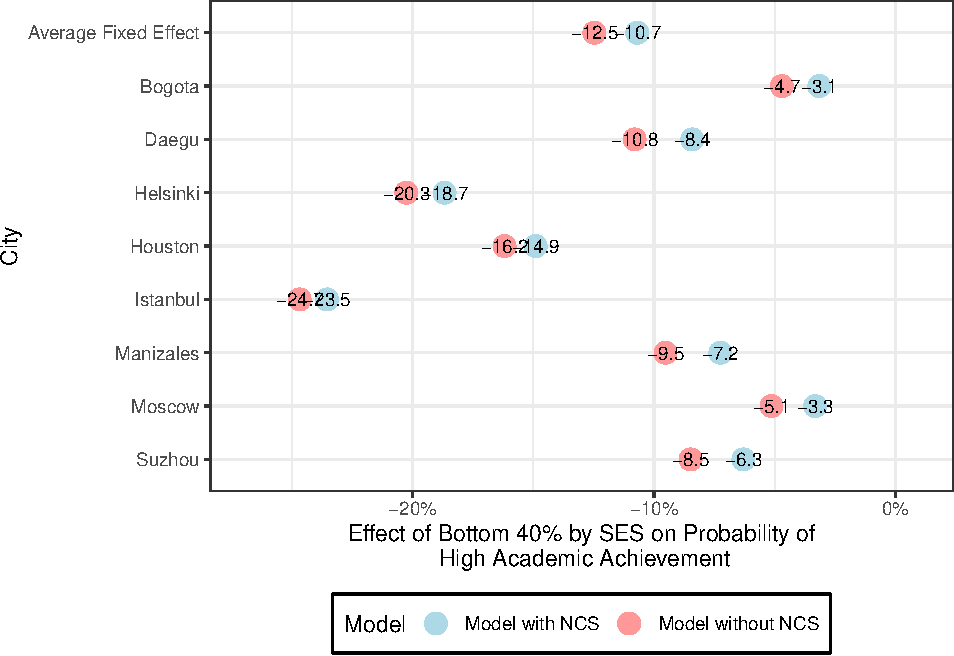
\includegraphics{ncs_and_academic_achievementRmd_files/figure-latex/reduce the gap-1.pdf}
\caption{Comparison of the effect of SES (Bottom 40\%) on Academic
Achievement, multilevel models before and after accounting for
non-cognitive skills}
\end{figure}

\hypertarget{how-strong-are-the-effects-of-non-cognitive-skills-on-academic-performance}{%
\subsection{How Strong Are the Effects of Non-Cognitive Skills on
Academic
Performance?}\label{how-strong-are-the-effects-of-non-cognitive-skills-on-academic-performance}}

For students categorized within the high academic achievement bracket
(top 25\% in each city), the model indicated significant effect for the
intercept, meaning that for an average student in the sample there is
difference in the baseline probability of being a high achiever. The
model identified statistically significant effect of sex, with males
less likely to be high achievers. Migration background had no
significant effect on high academic achievement.

Finally, when it comes to the non-cognitive skills, open mindedness and
task performance positively affect high achievement. As such, increase
in task performance on 1 standard deviation would result in increasing
the probability of high achievement by 4\%. Open mindedness, another
critical skill for academic performance, with one increase in its
standard deviation results in the increased likelihood of high
achievement by 3\%.

Emotional regulation and collaboration also show statistically
significant effects on academic achievement, though their direction
appears to be somewhat counter-intuitive. As such, they negatively
affect the probability of high performance. As an example, increase on 1
standard deviation in collaboration would decrease the likelihood of
high achievement by 2\%, whereas in emotional regulation on 1\%. An
analysis carried out further in this paper aims to unpack more the
reasons behind this observed pattern. Finally, engaging with others does
not have a statistically significant effect on academic performance. The
results of the fixed effect part of the multilevel model are presented
in Table 4.

\global\setlength{\Oldarrayrulewidth}{\arrayrulewidth}

\global\setlength{\Oldtabcolsep}{\tabcolsep}

\setlength{\tabcolsep}{0pt}

\renewcommand*{\arraystretch}{1.5}



\providecommand{\ascline}[3]{\noalign{\global\arrayrulewidth #1}\arrayrulecolor[HTML]{#2}\cline{#3}}

\begin{longtable}[c]{|p{1.77in}|p{0.75in}|p{1.07in}|p{0.82in}}

\caption{Multilevel\ regressions\ of\ probability\ of\ high\ achievement\ 
with\ random\ slopes\ of\ non-cognitive\ skills}\\

\ascline{1pt}{000000}{1-4}

\multicolumn{1}{>{\raggedright}m{\dimexpr 1.77in+0\tabcolsep}}{\textcolor[HTML]{000000}{\fontsize{11}{11}\selectfont{\global\setmainfont{Helvetica}{\textbf{Characteristic}}}}} & \multicolumn{1}{>{\centering}m{\dimexpr 0.75in+0\tabcolsep}}{\textcolor[HTML]{000000}{\fontsize{11}{11}\selectfont{\global\setmainfont{Helvetica}{\textbf{Beta}}}}} & \multicolumn{1}{>{\centering}m{\dimexpr 1.07in+0\tabcolsep}}{\textcolor[HTML]{000000}{\fontsize{11}{11}\selectfont{\global\setmainfont{Helvetica}{\textbf{95\%\ CI}}}}\textcolor[HTML]{000000}{\fontsize{11}{11}\selectfont{\global\setmainfont{Helvetica}{\textsuperscript{1}}}}} & \multicolumn{1}{>{\centering}m{\dimexpr 0.82in+0\tabcolsep}}{\textcolor[HTML]{000000}{\fontsize{11}{11}\selectfont{\global\setmainfont{Helvetica}{\textbf{p-value}}}}} \\

\ascline{1pt}{000000}{1-4}\endfirsthead \caption[]{Multilevel\ regressions\ of\ probability\ of\ high\ achievement\ 
with\ random\ slopes\ of\ non-cognitive\ skills}\\

\ascline{1pt}{000000}{1-4}

\multicolumn{1}{>{\raggedright}m{\dimexpr 1.77in+0\tabcolsep}}{\textcolor[HTML]{000000}{\fontsize{11}{11}\selectfont{\global\setmainfont{Helvetica}{\textbf{Characteristic}}}}} & \multicolumn{1}{>{\centering}m{\dimexpr 0.75in+0\tabcolsep}}{\textcolor[HTML]{000000}{\fontsize{11}{11}\selectfont{\global\setmainfont{Helvetica}{\textbf{Beta}}}}} & \multicolumn{1}{>{\centering}m{\dimexpr 1.07in+0\tabcolsep}}{\textcolor[HTML]{000000}{\fontsize{11}{11}\selectfont{\global\setmainfont{Helvetica}{\textbf{95\%\ CI}}}}\textcolor[HTML]{000000}{\fontsize{11}{11}\selectfont{\global\setmainfont{Helvetica}{\textsuperscript{1}}}}} & \multicolumn{1}{>{\centering}m{\dimexpr 0.82in+0\tabcolsep}}{\textcolor[HTML]{000000}{\fontsize{11}{11}\selectfont{\global\setmainfont{Helvetica}{\textbf{p-value}}}}} \\

\ascline{1pt}{000000}{1-4}\endhead



\multicolumn{4}{>{\raggedright}m{\dimexpr 4.41in+6\tabcolsep}}{\textcolor[HTML]{000000}{\fontsize{11}{11}\selectfont{\global\setmainfont{Helvetica}{\textsuperscript{1}}}}\textcolor[HTML]{000000}{\fontsize{11}{11}\selectfont{\global\setmainfont{Helvetica}{CI\ =\ Confidence\ Interval}}}} \\

\endfoot



\multicolumn{1}{>{\raggedright}p{\dimexpr 1.77in+0\tabcolsep}}{\textcolor[HTML]{000000}{\fontsize{11}{11}\selectfont{\global\setmainfont{Helvetica}{(Intercept)}}}} & \multicolumn{1}{>{\centering}p{\dimexpr 0.75in+0\tabcolsep}}{\textcolor[HTML]{000000}{\fontsize{11}{11}\selectfont{\global\setmainfont{Helvetica}{0.20}}}} & \multicolumn{1}{>{\centering}p{\dimexpr 1.07in+0\tabcolsep}}{\textcolor[HTML]{000000}{\fontsize{11}{11}\selectfont{\global\setmainfont{Helvetica}{0.09,\ 0.32}}}} & \multicolumn{1}{>{\centering}p{\dimexpr 0.82in+0\tabcolsep}}{\textcolor[HTML]{000000}{\fontsize{11}{11}\selectfont{\global\setmainfont{Helvetica}{0.015}}}} \\





\multicolumn{1}{>{\raggedright}p{\dimexpr 1.77in+0\tabcolsep}}{\textcolor[HTML]{000000}{\fontsize{11}{11}\selectfont{\global\setmainfont{Helvetica}{Sex}}}} & \multicolumn{1}{>{\centering}p{\dimexpr 0.75in+0\tabcolsep}}{\textcolor[HTML]{000000}{\fontsize{11}{11}\selectfont{\global\setmainfont{Helvetica}{}}}} & \multicolumn{1}{>{\centering}p{\dimexpr 1.07in+0\tabcolsep}}{\textcolor[HTML]{000000}{\fontsize{11}{11}\selectfont{\global\setmainfont{Helvetica}{}}}} & \multicolumn{1}{>{\centering}p{\dimexpr 0.82in+0\tabcolsep}}{\textcolor[HTML]{000000}{\fontsize{11}{11}\selectfont{\global\setmainfont{Helvetica}{}}}} \\





\multicolumn{1}{>{\raggedright}p{\dimexpr 1.77in+0\tabcolsep}}{\textcolor[HTML]{000000}{\fontsize{11}{11}\selectfont{\global\setmainfont{Helvetica}{Female}}}} & \multicolumn{1}{>{\centering}p{\dimexpr 0.75in+0\tabcolsep}}{\textcolor[HTML]{000000}{\fontsize{11}{11}\selectfont{\global\setmainfont{Helvetica}{—}}}} & \multicolumn{1}{>{\centering}p{\dimexpr 1.07in+0\tabcolsep}}{\textcolor[HTML]{000000}{\fontsize{11}{11}\selectfont{\global\setmainfont{Helvetica}{—}}}} & \multicolumn{1}{>{\centering}p{\dimexpr 0.82in+0\tabcolsep}}{\textcolor[HTML]{000000}{\fontsize{11}{11}\selectfont{\global\setmainfont{Helvetica}{}}}} \\





\multicolumn{1}{>{\raggedright}p{\dimexpr 1.77in+0\tabcolsep}}{\textcolor[HTML]{000000}{\fontsize{11}{11}\selectfont{\global\setmainfont{Helvetica}{Male}}}} & \multicolumn{1}{>{\centering}p{\dimexpr 0.75in+0\tabcolsep}}{\textcolor[HTML]{000000}{\fontsize{11}{11}\selectfont{\global\setmainfont{Helvetica}{-0.04}}}} & \multicolumn{1}{>{\centering}p{\dimexpr 1.07in+0\tabcolsep}}{\textcolor[HTML]{000000}{\fontsize{11}{11}\selectfont{\global\setmainfont{Helvetica}{-0.05,\ -0.04}}}} & \multicolumn{1}{>{\centering}p{\dimexpr 0.82in+0\tabcolsep}}{\textcolor[HTML]{000000}{\fontsize{11}{11}\selectfont{\global\setmainfont{Helvetica}{<0.001}}}} \\





\multicolumn{1}{>{\raggedright}p{\dimexpr 1.77in+0\tabcolsep}}{\textcolor[HTML]{000000}{\fontsize{11}{11}\selectfont{\global\setmainfont{Helvetica}{Migration\ Background}}}} & \multicolumn{1}{>{\centering}p{\dimexpr 0.75in+0\tabcolsep}}{\textcolor[HTML]{000000}{\fontsize{11}{11}\selectfont{\global\setmainfont{Helvetica}{}}}} & \multicolumn{1}{>{\centering}p{\dimexpr 1.07in+0\tabcolsep}}{\textcolor[HTML]{000000}{\fontsize{11}{11}\selectfont{\global\setmainfont{Helvetica}{}}}} & \multicolumn{1}{>{\centering}p{\dimexpr 0.82in+0\tabcolsep}}{\textcolor[HTML]{000000}{\fontsize{11}{11}\selectfont{\global\setmainfont{Helvetica}{}}}} \\





\multicolumn{1}{>{\raggedright}p{\dimexpr 1.77in+0\tabcolsep}}{\textcolor[HTML]{000000}{\fontsize{11}{11}\selectfont{\global\setmainfont{Helvetica}{0}}}} & \multicolumn{1}{>{\centering}p{\dimexpr 0.75in+0\tabcolsep}}{\textcolor[HTML]{000000}{\fontsize{11}{11}\selectfont{\global\setmainfont{Helvetica}{—}}}} & \multicolumn{1}{>{\centering}p{\dimexpr 1.07in+0\tabcolsep}}{\textcolor[HTML]{000000}{\fontsize{11}{11}\selectfont{\global\setmainfont{Helvetica}{—}}}} & \multicolumn{1}{>{\centering}p{\dimexpr 0.82in+0\tabcolsep}}{\textcolor[HTML]{000000}{\fontsize{11}{11}\selectfont{\global\setmainfont{Helvetica}{}}}} \\





\multicolumn{1}{>{\raggedright}p{\dimexpr 1.77in+0\tabcolsep}}{\textcolor[HTML]{000000}{\fontsize{11}{11}\selectfont{\global\setmainfont{Helvetica}{1}}}} & \multicolumn{1}{>{\centering}p{\dimexpr 0.75in+0\tabcolsep}}{\textcolor[HTML]{000000}{\fontsize{11}{11}\selectfont{\global\setmainfont{Helvetica}{0.00}}}} & \multicolumn{1}{>{\centering}p{\dimexpr 1.07in+0\tabcolsep}}{\textcolor[HTML]{000000}{\fontsize{11}{11}\selectfont{\global\setmainfont{Helvetica}{-0.01,\ 0.01}}}} & \multicolumn{1}{>{\centering}p{\dimexpr 0.82in+0\tabcolsep}}{\textcolor[HTML]{000000}{\fontsize{11}{11}\selectfont{\global\setmainfont{Helvetica}{0.8}}}} \\





\multicolumn{1}{>{\raggedright}p{\dimexpr 1.77in+0\tabcolsep}}{\textcolor[HTML]{000000}{\fontsize{11}{11}\selectfont{\global\setmainfont{Helvetica}{Open\ Mindedness}}}} & \multicolumn{1}{>{\centering}p{\dimexpr 0.75in+0\tabcolsep}}{\textcolor[HTML]{000000}{\fontsize{11}{11}\selectfont{\global\setmainfont{Helvetica}{0.03}}}} & \multicolumn{1}{>{\centering}p{\dimexpr 1.07in+0\tabcolsep}}{\textcolor[HTML]{000000}{\fontsize{11}{11}\selectfont{\global\setmainfont{Helvetica}{0.02,\ 0.03}}}} & \multicolumn{1}{>{\centering}p{\dimexpr 0.82in+0\tabcolsep}}{\textcolor[HTML]{000000}{\fontsize{11}{11}\selectfont{\global\setmainfont{Helvetica}{<0.001}}}} \\





\multicolumn{1}{>{\raggedright}p{\dimexpr 1.77in+0\tabcolsep}}{\textcolor[HTML]{000000}{\fontsize{11}{11}\selectfont{\global\setmainfont{Helvetica}{Task\ Performance}}}} & \multicolumn{1}{>{\centering}p{\dimexpr 0.75in+0\tabcolsep}}{\textcolor[HTML]{000000}{\fontsize{11}{11}\selectfont{\global\setmainfont{Helvetica}{0.04}}}} & \multicolumn{1}{>{\centering}p{\dimexpr 1.07in+0\tabcolsep}}{\textcolor[HTML]{000000}{\fontsize{11}{11}\selectfont{\global\setmainfont{Helvetica}{0.04,\ 0.05}}}} & \multicolumn{1}{>{\centering}p{\dimexpr 0.82in+0\tabcolsep}}{\textcolor[HTML]{000000}{\fontsize{11}{11}\selectfont{\global\setmainfont{Helvetica}{<0.001}}}} \\





\multicolumn{1}{>{\raggedright}p{\dimexpr 1.77in+0\tabcolsep}}{\textcolor[HTML]{000000}{\fontsize{11}{11}\selectfont{\global\setmainfont{Helvetica}{Engaging\ with\ Others}}}} & \multicolumn{1}{>{\centering}p{\dimexpr 0.75in+0\tabcolsep}}{\textcolor[HTML]{000000}{\fontsize{11}{11}\selectfont{\global\setmainfont{Helvetica}{0.01}}}} & \multicolumn{1}{>{\centering}p{\dimexpr 1.07in+0\tabcolsep}}{\textcolor[HTML]{000000}{\fontsize{11}{11}\selectfont{\global\setmainfont{Helvetica}{0.00,\ 0.01}}}} & \multicolumn{1}{>{\centering}p{\dimexpr 0.82in+0\tabcolsep}}{\textcolor[HTML]{000000}{\fontsize{11}{11}\selectfont{\global\setmainfont{Helvetica}{0.11}}}} \\





\multicolumn{1}{>{\raggedright}p{\dimexpr 1.77in+0\tabcolsep}}{\textcolor[HTML]{000000}{\fontsize{11}{11}\selectfont{\global\setmainfont{Helvetica}{Collaboration}}}} & \multicolumn{1}{>{\centering}p{\dimexpr 0.75in+0\tabcolsep}}{\textcolor[HTML]{000000}{\fontsize{11}{11}\selectfont{\global\setmainfont{Helvetica}{-0.02}}}} & \multicolumn{1}{>{\centering}p{\dimexpr 1.07in+0\tabcolsep}}{\textcolor[HTML]{000000}{\fontsize{11}{11}\selectfont{\global\setmainfont{Helvetica}{-0.03,\ -0.01}}}} & \multicolumn{1}{>{\centering}p{\dimexpr 0.82in+0\tabcolsep}}{\textcolor[HTML]{000000}{\fontsize{11}{11}\selectfont{\global\setmainfont{Helvetica}{<0.001}}}} \\





\multicolumn{1}{>{\raggedright}p{\dimexpr 1.77in+0\tabcolsep}}{\textcolor[HTML]{000000}{\fontsize{11}{11}\selectfont{\global\setmainfont{Helvetica}{Emotional\ Regulation}}}} & \multicolumn{1}{>{\centering}p{\dimexpr 0.75in+0\tabcolsep}}{\textcolor[HTML]{000000}{\fontsize{11}{11}\selectfont{\global\setmainfont{Helvetica}{-0.01}}}} & \multicolumn{1}{>{\centering}p{\dimexpr 1.07in+0\tabcolsep}}{\textcolor[HTML]{000000}{\fontsize{11}{11}\selectfont{\global\setmainfont{Helvetica}{-0.02,\ -0.01}}}} & \multicolumn{1}{>{\centering}p{\dimexpr 0.82in+0\tabcolsep}}{\textcolor[HTML]{000000}{\fontsize{11}{11}\selectfont{\global\setmainfont{Helvetica}{<0.001}}}} \\

\ascline{1pt}{000000}{1-4}



\multicolumn{1}{>{\raggedright}p{\dimexpr 1.77in+0\tabcolsep}}{\textcolor[HTML]{000000}{\fontsize{11}{11}\selectfont{\global\setmainfont{Helvetica}{No.\ Obs.}}}} & \multicolumn{1}{>{\centering}p{\dimexpr 0.75in+0\tabcolsep}}{\textcolor[HTML]{000000}{\fontsize{11}{11}\selectfont{\global\setmainfont{Helvetica}{44,394}}}} & \multicolumn{1}{>{\centering}p{\dimexpr 1.07in+0\tabcolsep}}{\textcolor[HTML]{000000}{\fontsize{11}{11}\selectfont{\global\setmainfont{Helvetica}{}}}} & \multicolumn{1}{>{\centering}p{\dimexpr 0.82in+0\tabcolsep}}{\textcolor[HTML]{000000}{\fontsize{11}{11}\selectfont{\global\setmainfont{Helvetica}{}}}} \\

\ascline{1pt}{000000}{1-4}



\end{longtable}



\arrayrulecolor[HTML]{000000}

\global\setlength{\arrayrulewidth}{\Oldarrayrulewidth}

\global\setlength{\tabcolsep}{\Oldtabcolsep}

\renewcommand*{\arraystretch}{1}

It is also important to consider the variance partitioning coefficients
from the calculated multilevel model. Examining the variance
contributions by model predictors refers to one of the key advantages of
the multilevel model framework, as it allows to identify the areas where
most of the variability persists. As such, for high performers, the
random intercept attributable to the school ID nested within the city
accounted for 16.5\%, suggesting that the between-school and city
differences in high achievement are substantially pronounced. The
results emphasize that school-level factors refer to the major
contributors of variation in academic performance. Additionally,
within-age differences (we have two age cohorts, namely, 10- and
15-year-olds) account for 1\% of variation in non-cognitive skills.

When examining the random slopes associated with the interaction of city
and socio-economic status group on non-cognitive skills, we observed
variability in the impact of these skills on academic outcomes. First of
all, despite the effect sizes of non-cognitive skills are quite notable,
altogether, five characteristics have a very little explanatory power in
terms of heterogeneity observed in high achievement. However, this
should not be misinterpreted. Even though non-cognitive skills may not
vary widely across the sample (hence the low variance explained), where
they do vary, they make a significant difference. Notably, the
additional variance component due to the random slope of the intercept
across cities and SES groups accounted for 2.7\% for high performers,
pointing to the existing heterogeneity in the baseline achievement
levels across different SES groups within cities. The residual variance,
representing within-student variability not explained by the model,
accounted for 79\% for high performers, underscoring a consistent level
of individual differences in academic performance. The results are
presented in Table 5.

\setlength{\LTpost}{0mm}
\begin{longtable}{lllrr}
\toprule
Effect & Group & Term & VPC & Explained Variance (\%) \\ 
\midrule\addlinespace[2.5pt]
Random Intercept & City * School ID & sd (Intercept) & 0.148 & 16.481 \\ 
Random Slope & City * SES Group & sd Emotional Regulation & 0.009 & 0.061 \\ 
Random Slope & City * SES Group & sd Collaboration & 0.013 & 0.127 \\ 
Random Slope & City * SES Group & sd Engaging with Others & 0.014 & 0.147 \\ 
Random Slope & City * SES Group & sd Task Performance & 0.012 & 0.108 \\ 
Random Slope & City * SES Group & sd Open Mindedness & 0.007 & 0.037 \\ 
Random Slope & City * SES Group & sd (Intercept) & 0.060 & 2.709 \\ 
Random Intercept & City & sd (Intercept) & 0.005 & 0.019 \\ 
Random Intercept & Cohort & sd (Intercept) & 0.042 & 1.327 \\ 
Random & Residual & sd Observation & 0.324 & 78.984 \\ 
\bottomrule
\end{longtable}
\begin{minipage}{\linewidth}
Source: Calculations of the authors based on the OECD SSES 2019 data.\\
\end{minipage}

\hypertarget{effect-of-non-cognitive-skills-on-the-academic-achievement-of-the-poorest-and-its-robustness-across-socio-economic-contexts}{%
\subsection{Effect of Non-Cognitive Skills on the Academic Achievement
of the Poorest and Its Robustness Across Socio-Economic
Contexts}\label{effect-of-non-cognitive-skills-on-the-academic-achievement-of-the-poorest-and-its-robustness-across-socio-economic-contexts}}

In assessing the impact of non-cognitive skills on high academic
achievement within socioeconomically disadvantaged groups, our
multilevel modeling revealed nuanced city-specific patterns. The
analysis, focusing on students in the bottom 40\% of the SES gradient,
highlighted the significant role of task performance and open-mindedness
as predictors of academic success (Figure 2). Task performance, with
positive slopes ranging from 3.5\% to 5.1\%, emerged as a robust
facilitator of high achievement, aligning with existing literature that
underscores its importance in educational outcomes (Dumfart \& Neubauer,
2016). Open-mindedness similarly exhibited positive associations,
suggesting that cognitive flexibility may enhance academic resilience, a
finding supported by most existing studies (Poropat, 2014).

However, the random slopes for emotional regulation and collaboration
presented a complex landscape. Both skills were consistently associated
with lower probabilities of high achievement---a result that stands in
contrast to conventional educational theories that typically associate
collaborative skills and emotional control with positive academic
performance. Specifically regarding emotional regulation, the observed
effect may arise due to the multidirectional impact of the facets. In
The Big Five framework, while anxiety facet of neuroticism is found to
be positively associated with academic motivation, depression and
vulnerability demonstrate an opposite effect (Apostolov \& Geldenhuys,
2022). These counterintuitive findings may also point to the potential
nonlinearity in the effects of these traits, as has been suggested by
recent inquiries into the intricate dynamics of social skills in
academic contexts (ref).

The substantial dataset of 44,394 individual observations lends
robustness to these insights, suggesting the findings may be
generalizable across similar urban educational settings. Future research
could further elucidate the mechanisms at play, potentially guiding the
design of targeted interventions that consider the rich tapestry of
individual and environmental factors influencing student achievement.

\begin{figure}
\centering
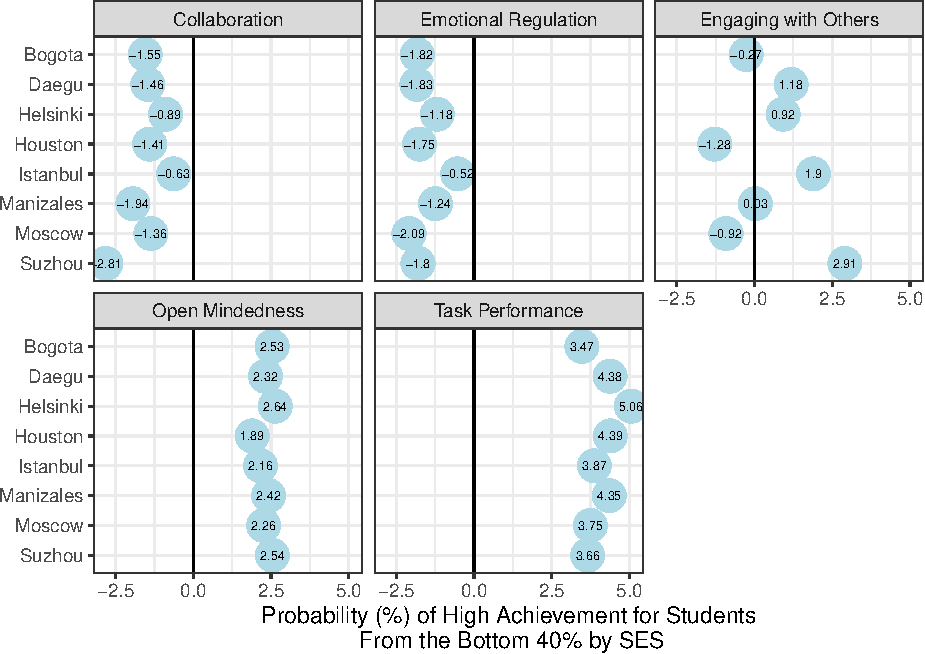
\includegraphics{ncs_and_academic_achievementRmd_files/figure-latex/mlm master chart-1.pdf}
\caption{Predicted Probability (Regression Coefficients) of Effect of
Non-Cognitive Skills on High Academic Achievement of Students from the
Bottom 40\% by SES}
\end{figure}

\hypertarget{how-equitable-are-returns-to-non-cognitive-skills}{%
\subsection{How Equitable Are Returns to Non-Cognitive
Skills?}\label{how-equitable-are-returns-to-non-cognitive-skills}}

While the previous analysis indeed affirms that investing into
development of non-cognitive skills, especially task performance and
open mindedness, produces substantial returns to academic performance
and can be used to facilitate human capital gains, it is still unclear
which socio-economic group would benefit the most from these
investments. In order to address this issue, we visually explore the
regression model on high performance, plotting the predicted
probabilities of the skills with the most profound and positive effect.
The charts on Figure 3 illustrate the predicted probabilities of high
academic achievement for students across three SES groups (Bottom 40\%,
Middle 50\%, and Top 10\%) as a function of two non-cognitive skills:
Task Performance and Open Mindedness. The slopes represent the
relationship between each skill and high achievement within each SES
group, disaggregated by city.

As indicated by Figure 3, higher levels of both task performance and
open mindedness consistently correlate with a higher probability of high
academic achievement across all cities and SES groups. However, visual
inspection of the skill slopes across SES groups and cities suggests
that the slopes are rather parallel, with the observed differences
arising due to the intercepts. In other words, the advantage of children
from the top 10\% richest households in the ways task performance and
open-mindedness affect their academic achievement is due to a higher
baseline probability of the wealthier students to be at the top of
distribution in learning outcomes. These differences at the intercept
could be due to various unobserved factors such as differences in prior
educational opportunities for children from the wealthier families,
disparities in parental education and social capital of families,
opportunities to maintain basic needs of the everyday life, such as
health and nutrition, etc. If richer kids always seem to have better
outcomes regardless of non-cognitive skills (as reflected by task
performance and open mindedness slopes), the benefits of these skills
are not distributed equally across SES groups. While non-cognitive
skills are necessary for academic success, they are not sufficient; the
advantages conferred by high SES (such as those listed above) might
amplify the effects of these skills.

\begin{figure}
\centering
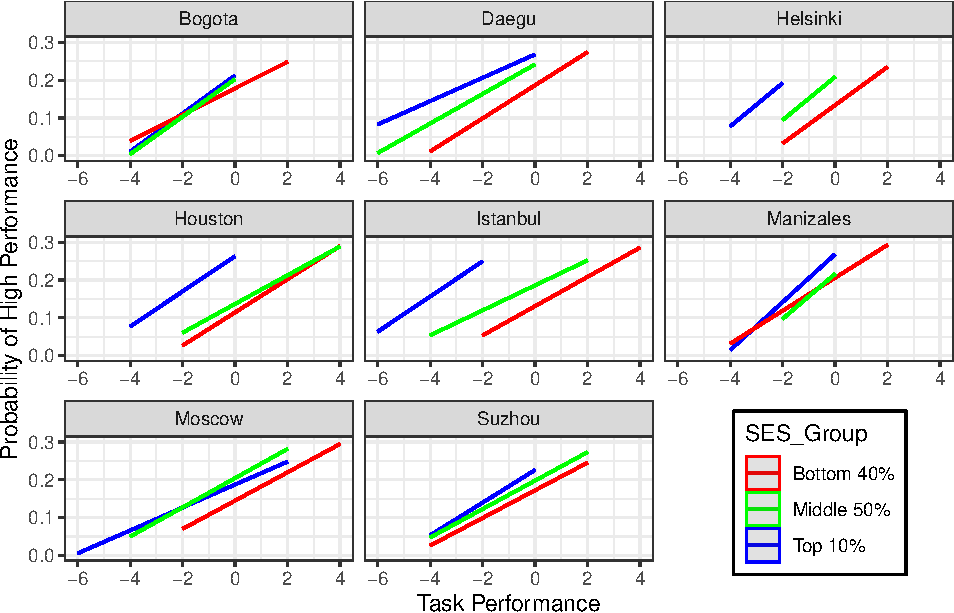
\includegraphics{ncs_and_academic_achievementRmd_files/figure-latex/scatter task perf-1.pdf}
\caption{Predicted Probabilities of Task Performance on High Academic
Achievement, by SES and City}
\end{figure}

\begin{figure}
\centering
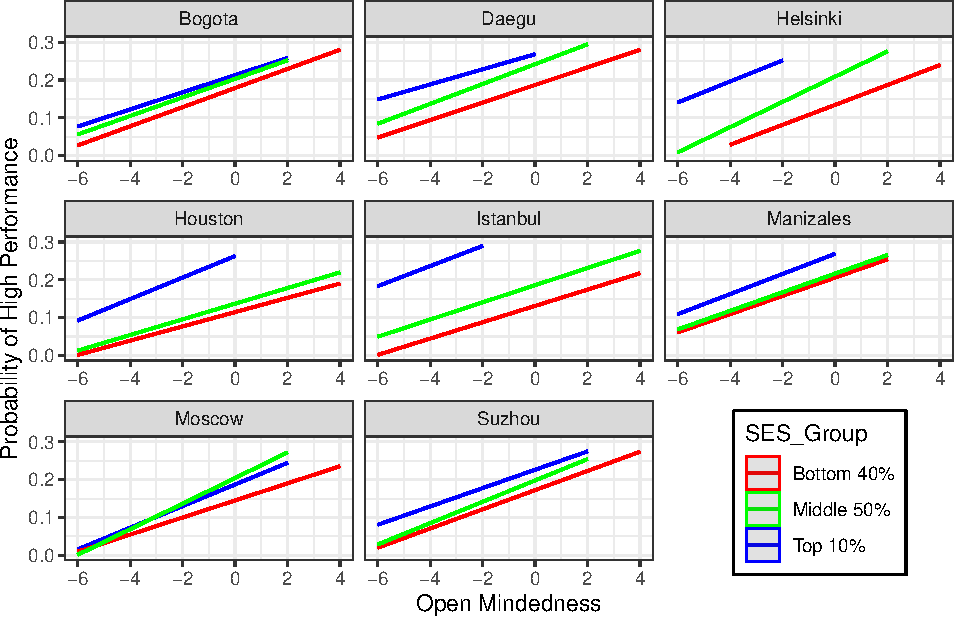
\includegraphics{ncs_and_academic_achievementRmd_files/figure-latex/scatter open-1.pdf}
\caption{Predicted Probabilities of Open Mindedness on High Academic
Achievement, by SES and City}
\end{figure}

\hypertarget{non-linearity-of-emotional-regulation-and-collaboration}{%
\subsection{Non-Linearity of Emotional Regulation and
Collaboration}\label{non-linearity-of-emotional-regulation-and-collaboration}}

At the final stage of our analysis, we are coming back to the effects of
emotional regulation and collaboration. We are testing the hypothesis
that these skills could present a nonlinear relationship with academic
performance and carry out an additional regression model that adopts
quadratic terms for these two variables. While the results for emotional
stability do not change, patterns identified in the relationship of
collaboration and academic achievement across SES groups and cities
present a compelling case.

Figures 4 and 5 visualizes the non-linear relationship between
collaboration and the probability of high academic achievement for
students across three SES groups in various cities. The non-linearity is
depicted by the curvature in the plotted lines for each SES group within
each city, indicating that the effect of collaboration on high
achievement varies at different levels of collaboration skill.

Across the cities, the relationship between collaboration and high
academic achievement shows a pronounced non-linear pattern, particularly
in Bogota, Daegu, Helsinki, and Istanbul, where the probability of high
performance initially increases with collaboration but begins to
decrease beyond a certain point. This inverted U-shaped curve suggests
that moderate levels of collaboration are most conducive to high
academic achievement, while both lower and higher levels are less so.
The peak of the curve represents the optimal point of collaboration that
maximizes the probability of being a high achiever. In contrast, cities
like Suzhou exhibit a different trend, with a consistent decline in the
probability of high performance as collaboration increases, highlighting
the variability of collaboration's impact on academic success across
different cultural and educational contexts.

The non-linear trends are particularly interesting when analyzed across
SES groups: for the Top 10\% SES group, the benefits of collaboration
are more pronounced at moderate levels but decline after a certain
threshold. The Middle 50\% SES group displays a similar but less
pronounced non-linear trend, suggesting that the balance of
collaboration for optimal academic outcomes also applies to this group
but with a wider range of effective collaboration levels. For the Bottom
40\% SES group, the increase in high performance probability is less
steep, and the decline starts at lower levels of collaboration compared
to the other SES groups. This could suggest that students from lower SES
backgrounds may have a narrower range of beneficial collaboration or
that other factors, such as access to resources or support systems, may
limit the positive effects of collaboration on their academic outcomes.

The observed patterns raise critical questions about the role of
collaboration in academic success and its potential interaction with
students' socio-economic backgrounds. While previous models suggested a
straightforward negative effect of emotional regulation on high
achievement, the intricate non-linear relationship revealed for
collaboration indicates that the impact of such non-cognitive skills on
academic performance is multifaceted and contingent upon the level of
skill exhibited.

\begin{figure}
\centering
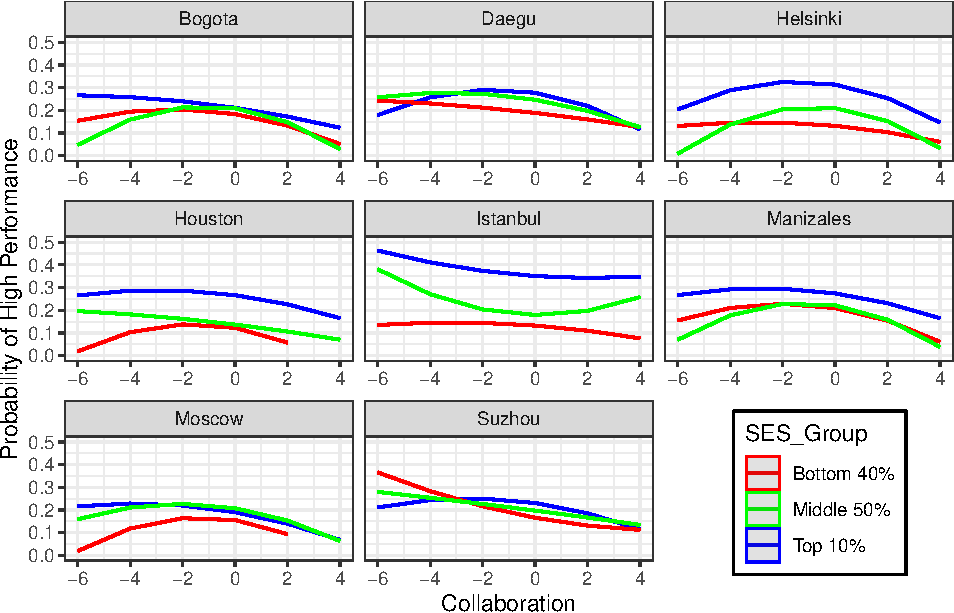
\includegraphics{ncs_and_academic_achievementRmd_files/figure-latex/collaboration-1.pdf}
\caption{Predicted Probability of Collaboration (Non-Linear Trend) on
High Academic Achievement, by SES and City}
\end{figure}

\hypertarget{research-limitations}{%
\section{Research Limitations}\label{research-limitations}}

Although our methodological approach allows us to account for different
unobserved effects associated with school and social status, it still
has several limitations. The first limitation is a natural consequence
of survey data. A problem, usually arising with the measurement of
personality traits in a survey setting, is reference bias which is a
tendency to respond to questionnaires in a socially acceptable way. For
instance, being more conscientious (hard-working, aim-oriented etc.) and
emotionally stable is more socially acceptable. Therefore, item response
for some of the Big Five categories, including conscientiousness and
neuroticism, may be unlikely to capture extremes (Morris et al., 2021).
Self-reports overstate at the bottom and top of the distribution of
non-cognitive skills (Edwards et al., 2022). Another issue is possible
reversed causality. For example, schooling intensity decreases emotional
stability (Dahmann \& Anger, 2018; Korthals et al., 2021), but increases
openness for students with lower SES (Dahmann \& Anger, 2018) Finally,
we do not control for cognitive abilities in our analysis due to lack of
proper measurements in the dataset.

\hypertarget{discussion}{%
\section{Discussion}\label{discussion}}

The pursuit of educational equity remains a paramount challenge in the
face of persistent socio-economic disparities. Children from poorer
households systematically demonstrate worse academic performance, being
significantly less presented among top achievers. Recognizing the
potential of non-cognitive skills to bridge the performance gap, this
analysis probes deeper into the influence of these skills on academic
outcomes.

First, our results suggest that non-cognitive skills are indeed linked
to academic performance. In the modified Big Five framework, our
analysis identified significant effects of task performance and
open-mindedness on academic performance, with robust findings for the
increase in the probability of high achievement. Task performance (or
conscientiousness in traditional Big Five) reflects diligence, attention
to details, and self-discipline, which are positively related to
individual productivity and the choice of appropriate study style,
leading to better academic outcomes (Poropat, 2014). Moreover, this
trait has been systematically shown to be associated with better
socio-economic decisions and outcomes in all life areas from attainment
and degree completion (Mendez \& Zamarro, 2017) to higher wages and
employment (Brunello \& Schlotter, 2011), longevity (Savelyev \& Tan,
2019), and lower probability of crime activity (J. Heckman et al.,
2006). Another critical non-cognitive skill for academic performance is
open mindedness (similar to openness to experience). Our analysis shows
that openness demonstrates rather stable effects on achievement for
students along the whole SES distribution, with the effect being a
little less pronounced in comparison to task performance. Open minded
students tend to gain more profound knowledge in their study areas,
which may result in better academic performance (McCrae \& Costa, 1997).
Emotional regulation and collaboration showed nontrivial effects
negatively affecting the probability of high achievement but did not
obtain high effect sizes. This result is different from those previously
discussed in the literature, since agreeableness is not usually
associated with any academic outcomes above primary school (Poropat,
2014). The effect of engaging with others (or extraversion) was not
statistically significant. We suppose that this skill may be more
relevant for contexts other than academic - for instance, labor market.

Second, we find that most of non-cognitive skills, including influential
task performance and open mindedness, demonstrate stable associations
with academic performance irrespective of the country in question. The
only exception is the skill of collaboration, which demonstrates a
significant, yet different non-linear trend in the relation with high
academic achievement. Given the complexity of these relationships,
further research is warranted to explore the underlying mechanisms
driving the non-linear effects of collaboration and to determine how
educational policies can be tailored to harness the benefits of
collaboration for all students, particularly those from lower SES
backgrounds.

Third, we do not find support for the hypothesis that non-cognitive
skills are more valuable for a particular SES group. For instance,
previous research, conducted on high school students and university
entrants suggests that openness is especially relevant for the
explanation of achievement for those with disadvantaged background
(Lundberg, 2013). We do not find empirical support for the critical
importance of openness for students from poorer households. In contrast,
high SES students seem to benefit more from having better non-cognitive
skills. Although non-cognitive skills are necessary for academic
success, children with the similar levels of task performance and
open-mindedness have higher chances of becoming high achievers if they
come from a more favorable socio-economic background. Therefore,
promoting the development of only non-cognitive skills in targeted
interventions is not enough. Further research is needed to explore the
mechanisms behind the observed disparities and to identify strategies
that can promote equity in the returns of non-cognitive skill
development.

Finally, we argue that the most influential non-cognitive skills can be
fostered through targeted educational policies, especially during early
stages of education. Since a significant part the model variance can be
attributed to the heterogeneity within schools, school-level
interventions on non-cognitive skill development within the established
curricula may be very effective to promote academic success. However,
the results observed for collaboration underscore the importance of a
more nuanced approach. Educational strategies and interventions designed
to enhance collaboration must consider the appropriate intensity and
context to ensure that they are effectively supporting academic success.
Same conclusion is applicable to emotional regulation. Although this
skill has been shown to positively influence academic scores acquired in
a high-stakes environment (e.g., during exams), in a less competitive
setting to achieve consistent performance, high emotional regulation may
have detrimental effects. In simple terms, one should care to be
academically successful. The exploration of non-linearity in these
relationships, as well as an investigation into moderating variables,
may yield insights into the multifaceted nature of skill development and
its consequences on learning.

\hypertarget{conclusions}{%
\section{Conclusions}\label{conclusions}}

This paper discusses educational inequality through the prism of
non-cognitive skills on a large sample of schoolchildren from 7
countries. Using multilevel modeling approach, which allows controlling
for fixed cohort, school, and country effects, we explore the impact of
a modified Big Five personality framework, consisting of task
performance, open mindedness, engaging with others, collaboration, and
emotional regulation, on the probability of entering top 25\% of
academic performance distribution among middle and high schoolers. The
results confirm that children from the poorest households systematically
lag behind in academic performance and tend to be underrepresented
amongst top performers. This can have substantial implications on their
human capital gains in a long term, as well as reproduction of poverty
patterns and lack of access to channels of social mobility.

Incorporating educational policies to enhance productive non-cognitive
skills has been repeatedly discussed as a potential mechanism of
reducing socio-economic gap in academic performance. Our results suggest
that non-cognitive skills are indeed very predictive of achievement,
although the magnitude of the effect varies by cultural and
socio-economic context of the country. The most influential positive
non-cognitive skills are task performance and open-mindedness, while
emotional regulation has a negative effect on academic achievement. A
non-trivial non-linear effect is observed for collaboration, suggesting
that both low and high manifestation of collaboration skills may be
detrimental for academic success.

Although non-cognitive skills indeed significantly reduce the effect of
SES on the probability of high achievement among schoolchildren, they
are not enough to close the achievement gap between the richest and the
poorest. High SES students with similar levels of skills are more likely
to become high achievers compared to low SES students due to the
disparity of educational opportunities and other unobserved background
factors. Therefore, performing targeted interventions, promoting
productive non-cognitive skills, may be important but not sufficient to
close the achievement gap.

\hypertarget{references}{%
\section*{References}\label{references}}
\addcontentsline{toc}{section}{References}

\hypertarget{refs}{}
\begin{CSLReferences}{1}{0}
\leavevmode\vadjust pre{\hypertarget{ref-Apostolov2022}{}}%
Apostolov, N., \& Geldenhuys, M. (2022). The role of neuroticism and
conscientious facets in academic motivation. \emph{Brain and Behavior},
\emph{12}(8). \url{https://doi.org/10.1002/brb3.2673}

\leavevmode\vadjust pre{\hypertarget{ref-Attanasio2020}{}}%
Attanasio, O., Blundell, R., Conti, G., \& Mason, G. (2020). Inequality
in socio-emotional skills: A cross-cohort comparison. \emph{Journal of
Public Economics}, \emph{191}, 104171.

\leavevmode\vadjust pre{\hypertarget{ref-avanesian2022}{}}%
Avanesian, G., Borovskaya, M., Ryzhova, V., Kirik, V., Egorova, V., \&
Bermous, A. (2022). Can we improve learning outcomes of schoolchildren
from the poorest families by investing into their non-cognitive skills?
Causal analysis using propensity score matching. \emph{Voprosy
Obrazovaniya / Educational Studies Moscow}, \emph{1}, 13--53.
\url{https://doi.org/10.17323/1814-9545-2022-1-13-53}

\leavevmode\vadjust pre{\hypertarget{ref-bates2015}{}}%
Bates, D., Mächler, M., Bolker, B., \& Walker, S. (2015). Fitting Linear
Mixed-Effects Models Using lme4. \emph{Journal of Statistical Software},
\emph{67}(1). \url{https://doi.org/10.18637/jss.v067.i01}

\leavevmode\vadjust pre{\hypertarget{ref-borghans2008}{}}%
Borghans, L., Duckworth, A. L., Heckman, J. J., \& Weel, B. ter. (2008).
The Economics and Psychology of Personality Traits. \emph{Journal of
Human Resources}, \emph{43}(4), 972--1059.
\url{https://doi.org/10.3368/jhr.43.4.972}

\leavevmode\vadjust pre{\hypertarget{ref-bratko2006}{}}%
Bratko, D., Chamorro-Premuzic, T., \& Saks, Z. (2006). Personality and
school performance: Incremental validity of self- and peer-ratings over
intelligence. \emph{Personality and Individual Differences},
\emph{41}(1), 131--142. \url{https://doi.org/10.1016/j.paid.2005.12.015}

\leavevmode\vadjust pre{\hypertarget{ref-brunello2011}{}}%
Brunello, G., \& Schlotter, M. (2011). Non-Cognitive Skills and
Personality Traits: Labour Market Relevance and Their Development in
Education \& Training Systems. \emph{SSRN Electronic Journal}.
\url{https://doi.org/10.2139/ssrn.1858066}

\leavevmode\vadjust pre{\hypertarget{ref-chamorro-premuzic2003}{}}%
Chamorro-Premuzic, T., \& Furnham, A. (2003). Personality predicts
academic performance: Evidence from two longitudinal university samples.
\emph{Journal of Research in Personality}, \emph{37}(4), 319--338.
\url{https://doi.org/10.1016/s0092-6566(02)00578-0}

\leavevmode\vadjust pre{\hypertarget{ref-conard2006}{}}%
Conard, M. A. (2006). Aptitude is not enough: How personality and
behavior predict academic performance. \emph{Journal of Research in
Personality}, \emph{40}(3), 339--346.
\url{https://doi.org/10.1016/j.jrp.2004.10.003}

\leavevmode\vadjust pre{\hypertarget{ref-cunha2007}{}}%
Cunha, F., \& Heckman, J. (2007). \emph{The technology of skill
formation}. \url{https://doi.org/10.3386/w12840}

\leavevmode\vadjust pre{\hypertarget{ref-cunha2008}{}}%
Cunha, F., \& Heckman, J. J. (2008). Formulating, Identifying and
Estimating the Technology of Cognitive and Noncognitive Skill Formation.
\emph{Journal of Human Resources}, \emph{43}(4), 738--782.
\url{https://doi.org/10.1353/jhr.2008.0019}

\leavevmode\vadjust pre{\hypertarget{ref-Dahmann2018}{}}%
Dahmann, S. C., \& Anger, S. (2018). \emph{Cross-fertilizing gains or
crowding out? Schooling intensity and noncognitive skills}. No.
2018-065.

\leavevmode\vadjust pre{\hypertarget{ref-deraad1996b}{}}%
De Raad, B., \& Schouwenburg, H. C. (1996). Personality in learning and
education: a review. \emph{European Journal of Personality},
\emph{10}(5), 303--336.
\url{https://doi.org/10.1002/(sici)1099-0984(199612)10:5\%3C303::aid-per262\%3E3.0.co;2-2}

\leavevmode\vadjust pre{\hypertarget{ref-ditton2018}{}}%
Ditton, H., Bayer, M., \& Wohlkinger, F. (2018). Structural and
motivational mechanisms of academic achievement: a mediation model of
social{-}background effects on academic achievement. \emph{The British
Journal of Sociology}, \emph{70}(4), 1276--1296.
\url{https://doi.org/10.1111/1468-4446.12506}

\leavevmode\vadjust pre{\hypertarget{ref-dumfart2016}{}}%
Dumfart, B., \& Neubauer, A. C. (2016). Conscientiousness Is the Most
Powerful Noncognitive Predictor of School Achievement in Adolescents.
\emph{Journal of Individual Differences}, \emph{37}(1), 8--15.
\url{https://doi.org/10.1027/1614-0001/a000182}

\leavevmode\vadjust pre{\hypertarget{ref-edwards2022}{}}%
Edwards, R., Gibson, R., Harmon, C., \& Schurer, S. (2022).
First-in-their-family students at university: Can non-cognitive skills
compensate for social origin? \emph{Economics of Education Review},
\emph{91}, 102318.
\url{https://doi.org/10.1016/j.econedurev.2022.102318}

\leavevmode\vadjust pre{\hypertarget{ref-Elkins2020}{}}%
Elkins, R., \& Schurer, S. (2020). Exploring the role of parental
engagement in non-cognitive skill development over the lifecourse.
\emph{Journal of Population Economics}, \emph{33}(3), 957--1004.

\leavevmode\vadjust pre{\hypertarget{ref-erikson2016}{}}%
Erikson, R. (2016). Is it enough to be bright? Parental background,
cognitive ability and educational attainment. \emph{European Societies},
\emph{18}(2), 117--135.
\url{https://doi.org/10.1080/14616696.2016.1141306}

\leavevmode\vadjust pre{\hypertarget{ref-feng2022}{}}%
Feng, S., Han, Y., Heckman, J. J., \& Kautz, T. (2022). Comparing the
reliability and predictive power of child, teacher, and guardian reports
of noncognitive skills. \emph{Proceedings of the National Academy of
Sciences}, \emph{119}(6). \url{https://doi.org/10.1073/pnas.2113992119}

\leavevmode\vadjust pre{\hypertarget{ref-fletcher2016}{}}%
Fletcher, J., \& Wolfe, B. (2016). \emph{The importance of family income
in the formation and evolution of non-cognitive skills in childhood}.
\url{https://doi.org/10.3386/w22168}

\leavevmode\vadjust pre{\hypertarget{ref-gil-hernuxe1ndez2021}{}}%
Gil-Hernández, C. J. (2021). The (Unequal) Interplay Between Cognitive
and Noncognitive Skills in Early Educational Attainment. \emph{American
Behavioral Scientist}, \emph{65}(11), 1577--1598.
\url{https://doi.org/10.1177/0002764221996764}

\leavevmode\vadjust pre{\hypertarget{ref-heaven2012}{}}%
Heaven, P. C. L., \& Ciarrochi, J. (2012). When IQ is not everything:
Intelligence, personality and academic performance at school.
\emph{Personality and Individual Differences}, \emph{53}(4), 518--522.
\url{https://doi.org/10.1016/j.paid.2012.04.024}

\leavevmode\vadjust pre{\hypertarget{ref-heckman2000}{}}%
Heckman, J. J. (2000). Policies to foster human capital. \emph{Research
in Economics}, \emph{54}(1), 3--56.
\url{https://doi.org/10.1006/reec.1999.0225}

\leavevmode\vadjust pre{\hypertarget{ref-Heckman2014}{}}%
Heckman, J. J., \& Mosso, S. (2014). The economics of human development
and social mobility. \emph{Annual Review of Economics}, \emph{6}(1),
689--733.

\leavevmode\vadjust pre{\hypertarget{ref-heckman2013}{}}%
Heckman, J., \& Kautz, T. (2013). \emph{Fostering and measuring skills:
Interventions that improve character and cognition}.
\url{https://doi.org/10.3386/w19656}

\leavevmode\vadjust pre{\hypertarget{ref-heckman2006}{}}%
Heckman, J., Stixrud, J., \& Urzua, S. (2006). \emph{The effects of
cognitive and noncognitive abilities on labor market outcomes and social
behavior}. \url{https://doi.org/10.3386/w12006}

\leavevmode\vadjust pre{\hypertarget{ref-hindman2010}{}}%
Hindman, A. H., Skibbe, L. E., Miller, A., \& Zimmerman, M. (2010).
Ecological contexts and early learning: Contributions of child, family,
and classroom factors during Head Start, to literacy and mathematics
growth through first grade. \emph{Early Childhood Research Quarterly},
\emph{25}(2), 235--250.
\url{https://doi.org/10.1016/j.ecresq.2009.11.003}

\leavevmode\vadjust pre{\hypertarget{ref-Jackson2013}{}}%
Jackson, M. (Ed.). (2013). \emph{Determined to succeed?} Stanford
University Press.
\url{https://doi.org/10.11126/stanford/9780804783026.001.0001}

\leavevmode\vadjust pre{\hypertarget{ref-kline1971}{}}%
Kline, P., \& Gale, A. (1971). EXTRAVERSION, NEUROTICISM AND PERFORMANCE
IN A PSYCHOLOGY EXAMINATION. \emph{British Journal of Educational
Psychology}, \emph{41}(1), 90--94.
\url{https://doi.org/10.1111/j.2044-8279.1971.tb00662.x}

\leavevmode\vadjust pre{\hypertarget{ref-komarraju2011}{}}%
Komarraju, M., Karau, S. J., Schmeck, R. R., \& Avdic, A. (2011). The
Big Five personality traits, learning styles, and academic achievement.
\emph{Personality and Individual Differences}, \emph{51}(4), 472--477.
\url{https://doi.org/10.1016/j.paid.2011.04.019}

\leavevmode\vadjust pre{\hypertarget{ref-korthals2021}{}}%
Korthals, R., Schils, T., \& Borghans, L. (2021). Track placement and
the development of cognitive and non-cognitive skills. \emph{Education
Economics}, \emph{30}(5), 540--559.
\url{https://doi.org/10.1080/09645292.2021.2010277}

\leavevmode\vadjust pre{\hypertarget{ref-lee2018}{}}%
Lee, J., \& Stankov, L. (2018). Non-cognitive predictors of academic
achievement: Evidence from TIMSS and PISA. \emph{Learning and Individual
Differences}, \emph{65}, 50--64.
\url{https://doi.org/10.1016/j.lindif.2018.05.009}

\leavevmode\vadjust pre{\hypertarget{ref-liu2020}{}}%
Liu, A. (2020). Non-Cognitive skills and the growing achievement Gap.
\emph{Research in Social Stratification and Mobility}, \emph{69},
100546. \url{https://doi.org/10.1016/j.rssm.2020.100546}

\leavevmode\vadjust pre{\hypertarget{ref-lubbers2010}{}}%
Lubbers, M. J., Van Der Werf, M. P. C., Kuyper, H., \& Hendriks, A. A.
J. (2010). Does homework behavior mediate the relation between
personality and academic performance? \emph{Learning and Individual
Differences}, \emph{20}(3), 203--208.
\url{https://doi.org/10.1016/j.lindif.2010.01.005}

\leavevmode\vadjust pre{\hypertarget{ref-lundberg2013a}{}}%
Lundberg, S. (2013). The College Type: Personality and Educational
Inequality. \emph{Journal of Labor Economics}, \emph{31}(3), 421--441.
\url{https://doi.org/10.1086/671056}

\leavevmode\vadjust pre{\hypertarget{ref-marks2016}{}}%
Marks, G. N. (2016). The relative effects of socio-economic,
demographic, non-cognitive and cognitive influences on student
achievement in Australia. \emph{Learning and Individual Differences},
\emph{49}, 1--10. \url{https://doi.org/10.1016/j.lindif.2016.05.012}

\leavevmode\vadjust pre{\hypertarget{ref-mccrae1997}{}}%
McCrae, R. R., \& Costa, P. T. (1997). Personality trait structure as a
human universal. \emph{American Psychologist}, \emph{52}(5), 509--516.
\url{https://doi.org/10.1037/0003-066x.52.5.509}

\leavevmode\vadjust pre{\hypertarget{ref-mccrae1992}{}}%
McCrae, R. R., \& John, O. P. (1992). An Introduction to the
Five{-}Factor Model and Its Applications. \emph{Journal of Personality},
\emph{60}(2), 175--215.
\url{https://doi.org/10.1111/j.1467-6494.1992.tb00970.x}

\leavevmode\vadjust pre{\hypertarget{ref-mendez2017}{}}%
Mendez, I., \& Zamarro, G. (2017). The intergenerational transmission of
noncognitive skills and their effect on education and employment
outcomes. \emph{Journal of Population Economics}, \emph{31}(2),
521--560. \url{https://doi.org/10.1007/s00148-017-0661-0}

\leavevmode\vadjust pre{\hypertarget{ref-mishkevich2021}{}}%
Mishkevich, A. M. (2021). Relationship between personal characteristics
and the academic performance of high school students.
\emph{Psychological-Educational Studies}, \emph{13}(1), 101--116.
\url{https://doi.org/10.17759/psyedu.2021130107}

\leavevmode\vadjust pre{\hypertarget{ref-morris2021}{}}%
Morris, T. T., Davey Smith, G., Berg, G. van den, \& Davies, N. M.
(2021). Consistency of noncognitive skills and their relation to
educational outcomes in a UK cohort. \emph{Translational Psychiatry},
\emph{11}(1). \url{https://doi.org/10.1038/s41398-021-01661-8}

\leavevmode\vadjust pre{\hypertarget{ref-noftle2007a}{}}%
Noftle, E. E., \& Robins, R. W. (2007). Personality predictors of
academic outcomes: Big five correlates of GPA and SAT scores.
\emph{Journal of Personality and Social Psychology}, \emph{93}(1),
116--130. \url{https://doi.org/10.1037/0022-3514.93.1.116}

\leavevmode\vadjust pre{\hypertarget{ref-Nye2013}{}}%
Nye, J. V. C., Orel, E., \& Kochergina, E. (2013). Big five personality
traits and academic performance in russian universities. In \emph{Higher
School of Economics Research Paper No. WP BRP} (Vol. 10).

\leavevmode\vadjust pre{\hypertarget{ref-oconnor2007}{}}%
O'Connor, M. C., \& Paunonen, S. V. (2007). Big Five personality
predictors of post-secondary academic performance. \emph{Personality and
Individual Differences}, \emph{43}(5), 971--990.
\url{https://doi.org/10.1016/j.paid.2007.03.017}

\leavevmode\vadjust pre{\hypertarget{ref-oecd2021a}{}}%
OECD. (2021a). \emph{Beyond academic learning: First results from the
survey of social and emotional skills}. OECD.
\url{https://doi.org/10.1787/92a11084-en}

\leavevmode\vadjust pre{\hypertarget{ref-oecd2021b}{}}%
OECD. (2021b). \emph{OECD survey on social and emotional skills
technical report}. OECD.
\url{https://www.oecd.org/education/ceri/social-emotional-skills-study/sses-technical-report.pdf}

\leavevmode\vadjust pre{\hypertarget{ref-orel2018}{}}%
Orel, E., Brun, I., Kardanova, E., \& Antipkina, I. (2018).
Developmental Patterns of Cognitive and Non-Cognitive Skills of Russian
First-Graders. \emph{International Journal of Early Childhood},
\emph{50}(3), 297--314. \url{https://doi.org/10.1007/s13158-018-0226-8}

\leavevmode\vadjust pre{\hypertarget{ref-poropat2009}{}}%
Poropat, A. E. (2009). A meta-analysis of the five-factor model of
personality and academic performance. \emph{Psychological Bulletin},
\emph{135}(2), 322--338. \url{https://doi.org/10.1037/a0014996}

\leavevmode\vadjust pre{\hypertarget{ref-poropat2014}{}}%
Poropat, A. E. (2014). Other-rated personality and academic performance:
Evidence and implications. \emph{Learning and Individual Differences},
\emph{34}, 24--32. \url{https://doi.org/10.1016/j.lindif.2014.05.013}

\leavevmode\vadjust pre{\hypertarget{ref-reardon2016}{}}%
Reardon, S. F., \& Portilla, X. A. (2016). Recent Trends in Income,
Racial, and Ethnic School Readiness Gaps at Kindergarten Entry.
\emph{AERA Open}, \emph{2}(3), 233285841665734.
\url{https://doi.org/10.1177/2332858416657343}

\leavevmode\vadjust pre{\hypertarget{ref-richardson2012}{}}%
Richardson, M., Abraham, C., \& Bond, R. (2012). Psychological
correlates of university students' academic performance: A systematic
review and meta-analysis. \emph{Psychological Bulletin}, \emph{138}(2),
353--387. \url{https://doi.org/10.1037/a0026838}

\leavevmode\vadjust pre{\hypertarget{ref-rosander2014}{}}%
Rosander, P., \& Bäckström, M. (2014). Personality traits measured at
baseline can predict academic performance in upper secondary school
three years late. \emph{Scandinavian Journal of Psychology},
\emph{55}(6), 611--618. \url{https://doi.org/10.1111/sjop.12165}

\leavevmode\vadjust pre{\hypertarget{ref-savelyev2019}{}}%
Savelyev, P. A., \& Tan, K. T. K. (2019). Socioemotional Skills,
Education, and Health-Related Outcomes of High-Ability Individuals.
\emph{American Journal of Health Economics}, \emph{5}(2), 250--280.
\url{https://doi.org/10.1162/ajhe_a_00116}

\leavevmode\vadjust pre{\hypertarget{ref-shanahan2014}{}}%
Shanahan, M. J., Bauldry, S., Roberts, B. W., Macmillan, R., \& Russo,
R. (2014). Personality and the Reproduction of Social Class.
\emph{Social Forces}, \emph{93}(1), 209--240.
\url{https://doi.org/10.1093/sf/sou050}

\leavevmode\vadjust pre{\hypertarget{ref-smrtnikvitulic2012}{}}%
Smrtnik Vitulić, H., \& Zupančič, M. (2012). Robust and specific
personality traits as predictors of adolescents{'} final grades and GPA
at the end of compulsory schooling. \emph{European Journal of Psychology
of Education}, \emph{28}(4), 1181--1199.
\url{https://doi.org/10.1007/s10212-012-0161-2}

\leavevmode\vadjust pre{\hypertarget{ref-vonstumm2017}{}}%
Stumm, S. von. (2017). Socioeconomic status amplifies the achievement
gap throughout compulsory education independent of intelligence.
\emph{Intelligence}, \emph{60}, 57--62.
\url{https://doi.org/10.1016/j.intell.2016.11.006}

\leavevmode\vadjust pre{\hypertarget{ref-west2016}{}}%
West, M. R., Kraft, M. A., Finn, A. S., Martin, R. E., Duckworth, A. L.,
Gabrieli, C. F. O., \& Gabrieli, J. D. E. (2016). Promise and Paradox.
\emph{Educational Evaluation and Policy Analysis}, \emph{38}(1),
148--170. \url{https://doi.org/10.3102/0162373715597298}

\leavevmode\vadjust pre{\hypertarget{ref-zamarro2019}{}}%
Zamarro, G., Hitt, C., \& Mendez, I. (2019). When Students Don{'}t Care:
Reexamining International Differences in Achievement and Student Effort.
\emph{Journal of Human Capital}, \emph{13}(4), 519--552.
\url{https://doi.org/10.1086/705799}

\end{CSLReferences}

\end{document}
